\documentclass[8pt, handout=show,notes=show]{beamer}

\usepackage[utf8x]{inputenc}
\usepackage[T1]{fontenc}
\usepackage{wrapfig}
\usepackage{default}
\usetheme[width=2cm]{Goettingen}
\usepackage{amsmath}
\usecolortheme{rose}
\usepackage{enumerate}
\usepackage{graphicx}
\usepackage{wrapfig} 
\usepackage{amsmath}
\usepackage{lmodern}
\usepackage{subfigure}
\usepackage{float}


% \usepackage[colorlinks=true,urlcolor=blue,citecolor=green,linkcolor=blue,bookmarks=true]{hyperref}
\usepackage[french]{babel}
\author[]{Simon Carrignon \\ 
\vfill Encadrant: Nicolas Bred\`{e}che }
\institute[]{
	École~Pratique~des~Hautes~Études, \and TAO/LRI\\
	\pgfdeclareimage[height=0.5cm]{ephe}{../20110616-SoutenanceMemoire/images/logo_ephe_large.jpg} %declare logo image with an alias here 
	\pgfuseimage{ephe} \hfill \pgfdeclareimage[height=0.5cm]{inria}{../20110616-SoutenanceMemoire/images/taologo.jpg} %declare logo image with an alias here 
	\pgfuseimage{inria}
	
}

\usepackage[small]{caption}
% \DeclareLanguageMapping{american}{american-apa}
% \setbeamertemplate{caption}[numbered]
% \usepackage{subcaption}

% \usepackage{tikz}
% \usetikzlibrary{decorations.pathreplacing}
\useoutertheme{infolines}
% \logo{
\includegraphics[height=0.5cm]{../20110616-SoutenanceMemoire/images/logo_ephe_large.jpg}}
% 	\usepackage{wrapfig}
\usepackage{subfigure}
\usepackage[footheight=1em]{beamerthemeboxes}

\addfootboxtemplate{\color{black}}{\color{white}
\hspace{2em}Simon Carrignon \hfill\insertframenumber/\inserttotalframenumber\hspace{2em}\null}

\title{Specialization in a swarm of robots : impact of topologies}

\usepackage{algorithm}
\usepackage{algorithmic}

\usepackage[]{natbib}
\bibpunct{[}{]}{,}{a}{,}{,}
%%Repris du
%%Talk fait a l'EPHE le 16 juin 2011. 
%%Pour presentation du 7 octobre à TAO

\date{$20$ Octobre 2011}
\begin{document}
\begin{frame}
\maketitle

\end{frame}
	\newcommand{\imgSize}{4.2cm}

%%%------------------------------------------------------------------------
%%%----------------------------------------------------------------------
 \section{Introduction}
%%%----------------------------------------------------------------------
\begin{frame}{Autonomous agents, swarm intelligence, embodied evolution}
        \begin{figure}
		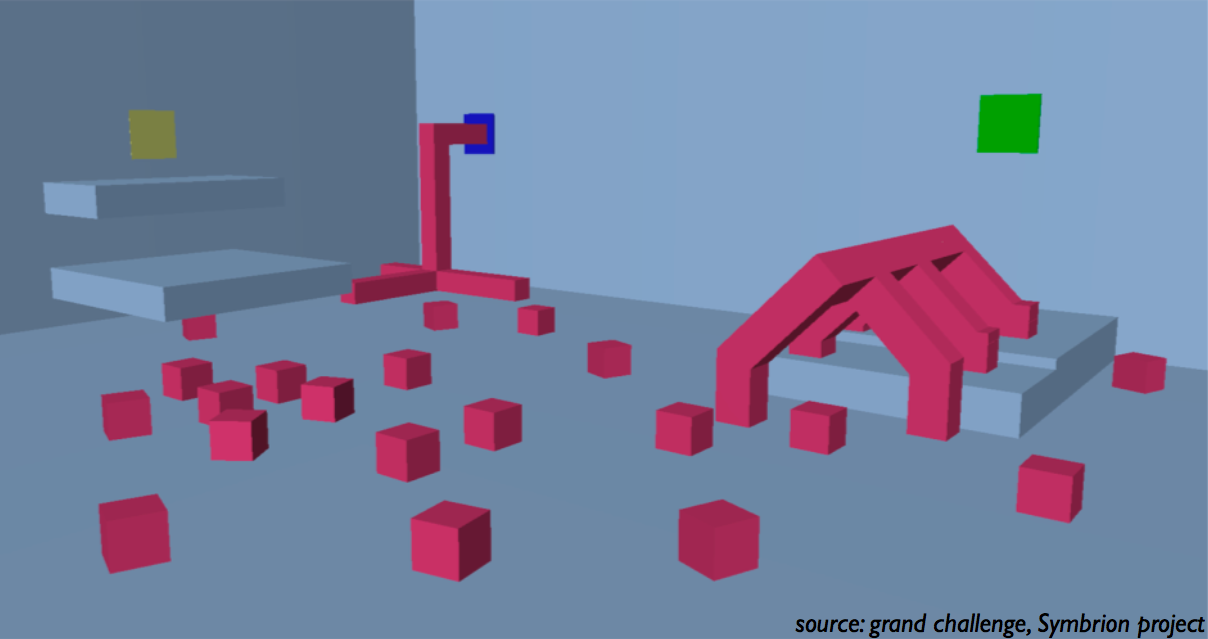
\includegraphics[height=3cm]{../20110616-SoutenanceMemoire/images/symbrion-gc1b.png}
        \end{figure}
	
	Swarm of autonomous agents with limited hardware abilities, in unknown, unpredictable and changing environments. 
	\begin{itemize}
		\item[$\rightarrow$] Goal: open-ended evolution with autonomous agents (online, onboard, distributed).
	\end{itemize}


\end{frame}
%%%----------------------------------------------------------------------
\subsection{mEDEA}
%%%----------------------------------------------------------------------
%%%%%%%%%%%%%%%%%%%%%%%%%%%%%%%%%%%%%%%%%%%%%%%%%%%555
%From jm and nicolas frame 

  \newcommand{\mEDEA}{

	\begin{itemize}
		\item Each agent contains:
		\begin{itemize}
			\item an active genome, used to control the agent,
			\item a list of stored genomes, received during one generation.
		\end{itemize}
		
		\item At each time step, each agent:
		\begin{itemize}
			\item broadcasts a copy of its active genome,
			\item stores genomes received from neighboring agents.
		\end{itemize}
		
		\item At the end of the current generation, each agent:
		\begin{itemize}
			\item "forgets" its active genome,
			\item randomly selects one stored genome as new active genome and mutate it a little bit,
			\item empties the list of stored genomes.
		\end{itemize}
	\end{itemize}

}


%------------------------------------------------------------
\begin{frame}{The "mEDEA" Algorithm}
\begin{figure}
 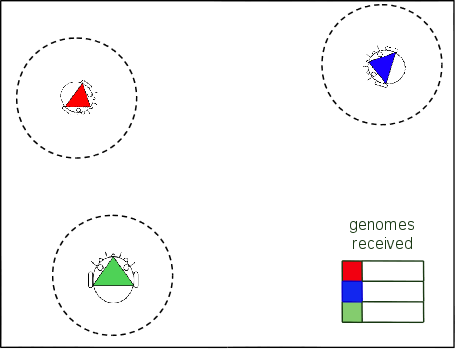
\includegraphics[height=3cm]{images/medea0}
\end{figure}

  \mEDEA

\end{frame}

%------------------------------------------------------------
\begin{frame}{The "mEDEA" Algorithm}\addtocounter{framenumber}{-1}
\begin{figure}
 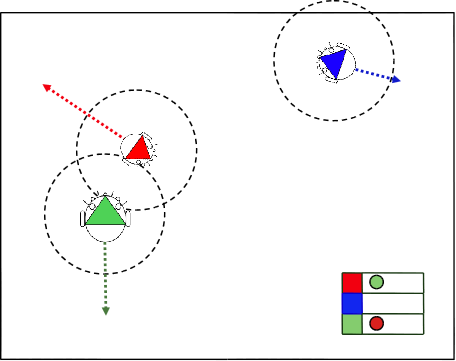
\includegraphics[height=3cm]{images/medea1}
\end{figure}
   \mEDEA
\end{frame}
%------------------------------------------------------------
\begin{frame}{The "mEDEA" Algorithm}\addtocounter{framenumber}{-1}
\begin{figure}
 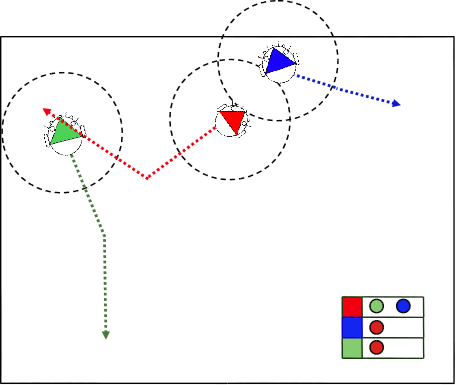
\includegraphics[height=3cm]{images/medea2}
\end{figure}
   \mEDEA
\end{frame}

%------------------------------------------------------------

\begin{frame}{The "mEDEA" Algorithm}\addtocounter{framenumber}{-1}
\begin{figure}
 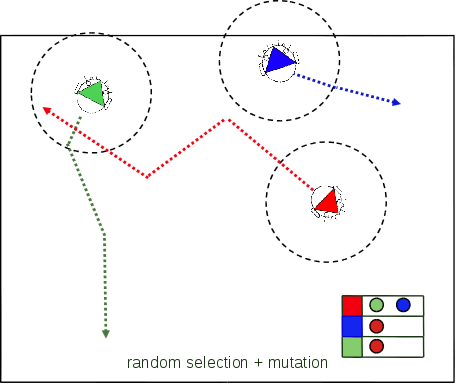
\includegraphics[height=3cm]{images/medea3}
\end{figure}
   \mEDEA
\end{frame}


%%%%%%%%%%%%%%%%%%%%%%%%%%%%%%%%%%



	
\begin{frame}{mEDEA }


\begin{figure}
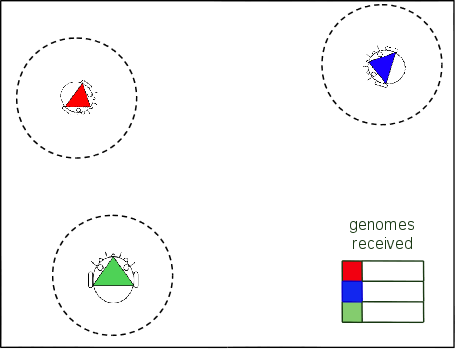
\includegraphics[height=3cm]{images/medea0}
\end{figure}
mEDEA, unsupervised, distributed evolution :
	\begin{itemize}
		\item Robust to environmental changes [PPSN2010] \nocite{bredeche11mcmds} 
		\item Works in real world [MCMDS2011] %\nocitep{montanier}
		\item Emergence of Altruism [ECAL2011]
	\end{itemize}

\vfill

Motivation : Study specialization and speciation in mEDEA




\end{frame}

%%%----------------------------------------------------------------------
%%%----------------------------------------------------------------------

\subsection{Speciation}

%%%----------------------------------------------------------------------
%%%----------------------------------------------------------------------

\begin{frame}{Speciation}
	\begin{columns}
		\column{.65\textwidth}
			An old problem since Darwin {\scriptsize \texttt [Darwin1856]} :
			\begin{itemize}
				\item allopatric {\scriptsize \texttt [Mayr1942]}
				\item sympatric  {\scriptsize \texttt [MaynardSmith1962] } : a hard way 
				\begin{quotation}
					\small
					[...] if disruptive selection is to lead to stable polymorphism, [..], the conditions which must be satisfied are severe. But they are of a kind which may often be satisfied in laboratory experiments, and wich may perhaps somteimes be met with in Nature.
				\end{quotation}

			\end{itemize}
		\column{.5\textwidth}
			\begin{figure}
				\subfigure[Allopatric speciation]{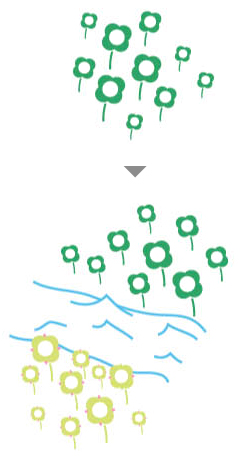
\includegraphics[width=.3\textwidth]{../20110616-SoutenanceMemoire/images/SpeciationAl}}	\label{figa:specAl} 
				\hspace{.2cm}
				\subfigure[Sympatric speciation]{
					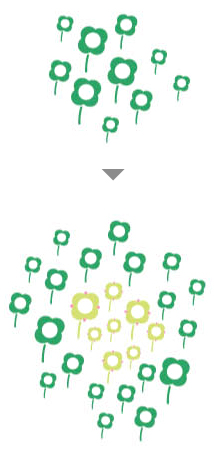
\includegraphics[width=.3\textwidth]{../20110616-SoutenanceMemoire/images/SpeciationSy}
				}	\label{figa:specSy} 
			% \caption{Diff. cas}
			\end{figure}
	\end{columns}
	\begin{alertblock}<3->{In a swarm of robot under evolution (sympatric case):}
		\begin{itemize}
		% 			\centering
			\item is speciation possible?
			\item in which conditions/mechanismes : topologie of the interaction's network.

		\end{itemize}
	\end{alertblock}
\end{frame}

%%%----------------------------------------------------------------------
%%%----------------------------------------------------------------------



%%%----------------------------------------------------------------------
%%%----------------------------------------------------------------------

\section{General settings}

\begin{frame}{Experimental Design}
	\begin{columns}[t]
		\column{0.45\textwidth}
			\begin{block}{The environment:}
				\begin{itemize}
					\item fixed number of agents,
					\item two sources of two kind,
				\end{itemize}
			\end{block}
		\column{0.45\textwidth}
			\begin{block}{Ability to forage:}
				\begin{itemize}
					\item a gene $g_{skill}$ which determine the "foraging skills" of an agent
				\end{itemize}
			\end{block}
	\end{columns}
	\begin{columns}
		\column{0.57\textwidth}
		\begin{block}{The foraging reward function: $F_{rwd}$}
			Quantity of energy agent can take :
			$F_{rwd,t}(i,Q) = f_{skill}\left(g_{s,i},T_Q\right)\alpha$%\times d_{penality}\left(h_{Q,t}\right)\times \alpha$
		\end{block}
	\end{columns}
	\begin{figure}
		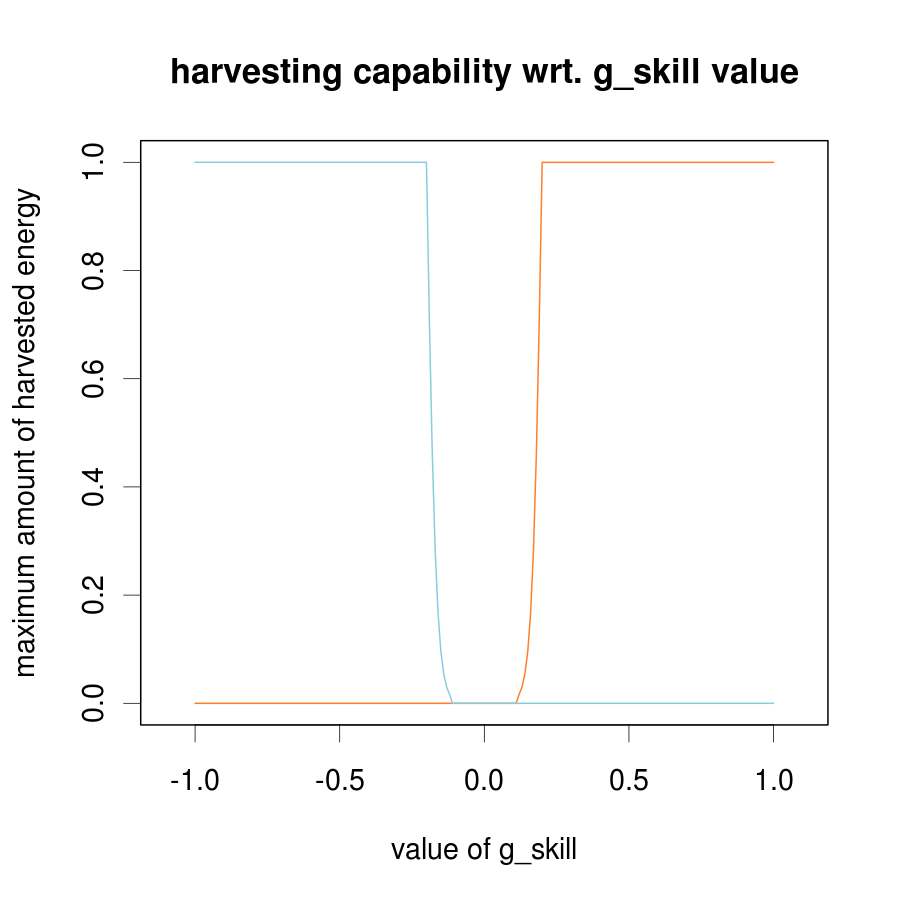
\includegraphics[width=.45\textwidth]{../images/sparsityEffect/f_skill}
	\end{figure}
\end{frame}
 
%%%----------------------------------------------------------------------
%%%----------------------------------------------------------------------


\section{Five topologies}
\subsection{Experimental design}
\begin{frame}{5 topologies}
	A simplified problem :
	\begin{itemize}
		\item no motion,
		\item 5 fixed topologies. 
	\end{itemize}

	\begin{table}[h]
		\begin{tabular}{l|c|c|}
			\scriptsize
			&robot disposition& resources disposition: \\
			\hline
			ENV0 &every robot can communicate& Full access\\\hline
			ENV1 &Chain & Full access\\\hline
			ENV2 &Chain & Limited access \\\hline
			ENV3&Two groups & Full access\\\hline
			ENV4&Two groups & Limited access 
		\end{tabular}
	\end{table}
	
	\renewcommand{\imgSize}{2cm}
	\small
	\begin{table}[h]
	\centering
		\begin{tabular}{lcc}
			&Full access&Limited access\\
			% \newline
			all linked&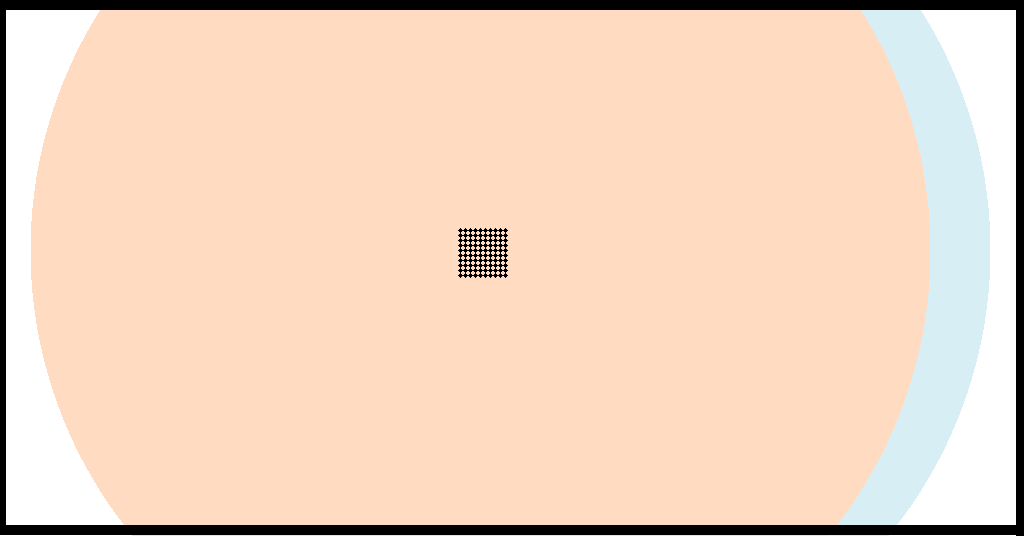
\includegraphics[width=\imgSize]{../images/5StaticEnv/environments/staticEnv0}&\\
			% \newline
			Chain&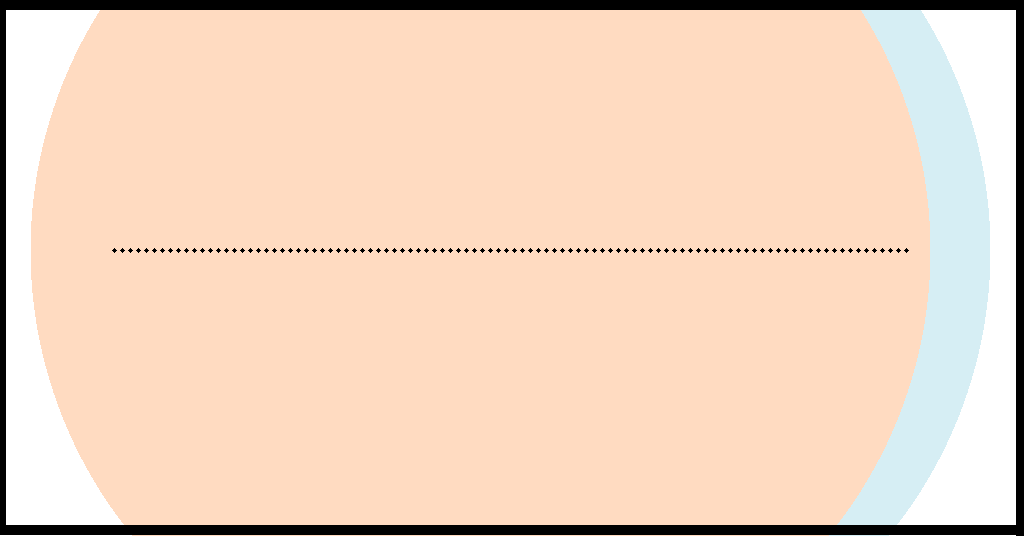
\includegraphics[width=\imgSize]{../images/5StaticEnv/environments/staticEnv1}&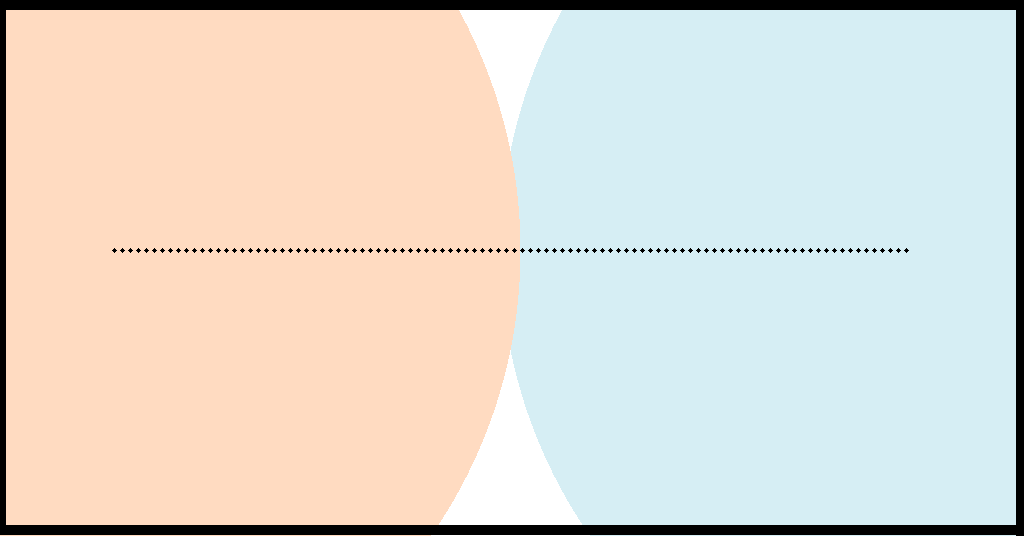
\includegraphics[width=\imgSize]{../images/5StaticEnv/environments/staticEnv2}\\
			Two groups&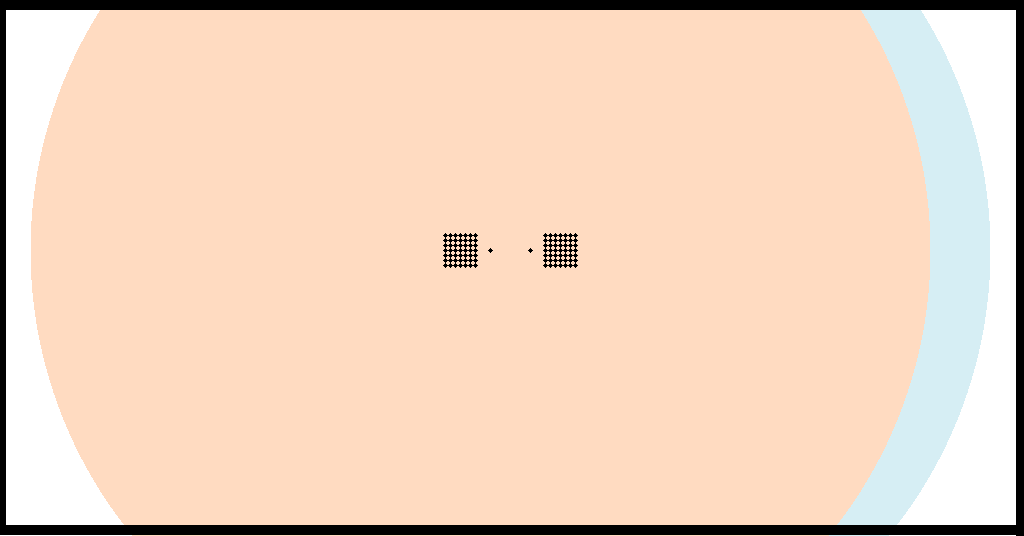
\includegraphics[width=\imgSize]{../images/5StaticEnv/environments/staticEnv3}&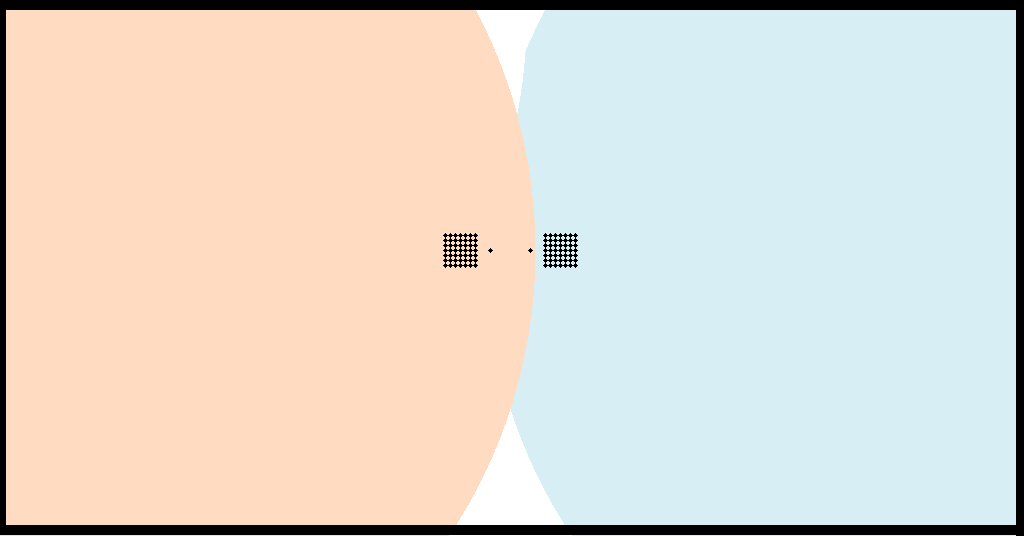
\includegraphics[width=\imgSize]{../images/5StaticEnv/environments/staticEnv4}\\
		% \newline
		\end{tabular}
	\label{tab:gt}

	\end{table}%
\end{frame} %%%---------------------------------------------------------------------- %%%---------------------------------------------------------------------- 
\subsection{Results} \begin{frame}{Results} \subsubsection{Each ressource can feed 50\% of the population:} When each ressource can feed 50\% of the population: \renewcommand{\imgSize}{3cm} % % 
% \begin{columns} % % 
% \column{.25\textwidth} % 	
\begin{figure} 
%
% 
% 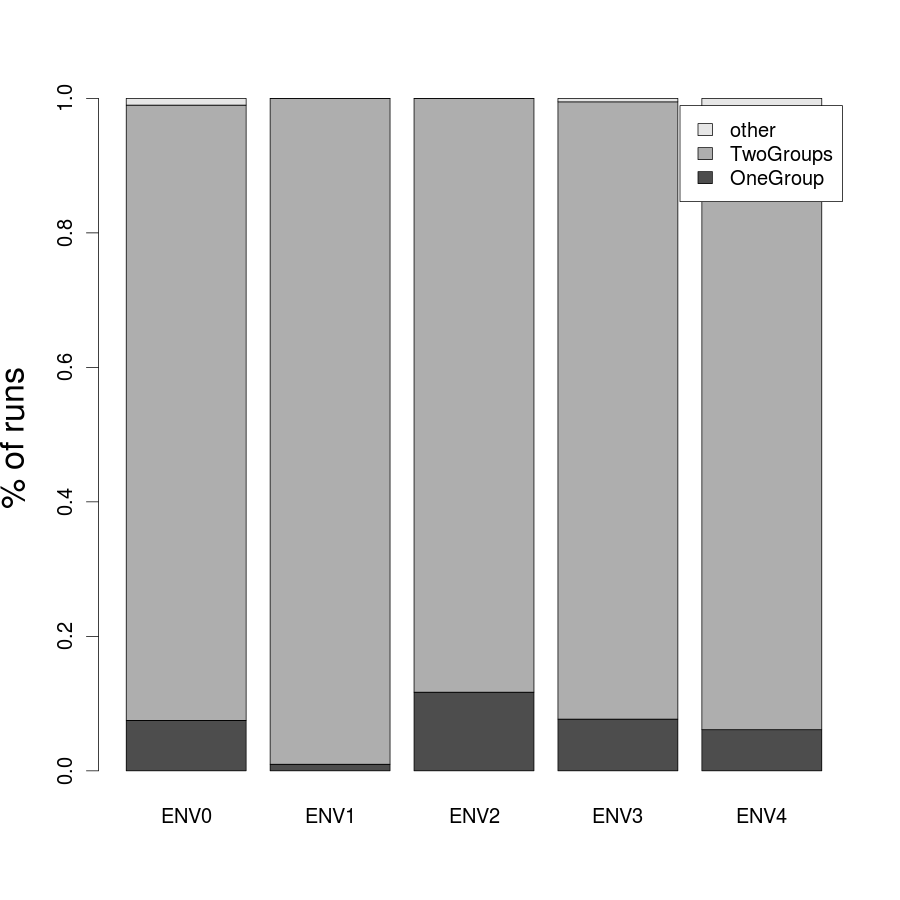
\includegraphics[width=\imgSize]{image
s/qualitative_distribution} % 	
\end{figure} % 
% \column{.7\textwidth} 
\begin{table}[H] \centering \begin{tabular}{ccc} &ENV1&ENV2\\ 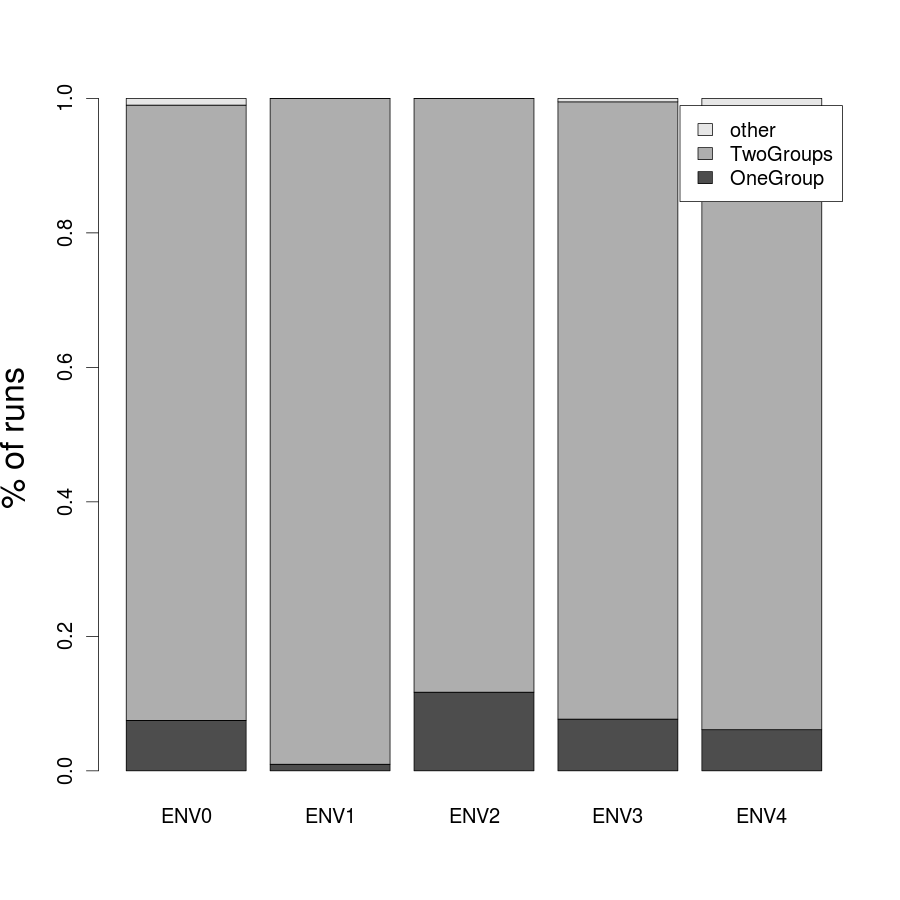
\includegraphics[width=\imgSize]{images/qualitative_distribution}& 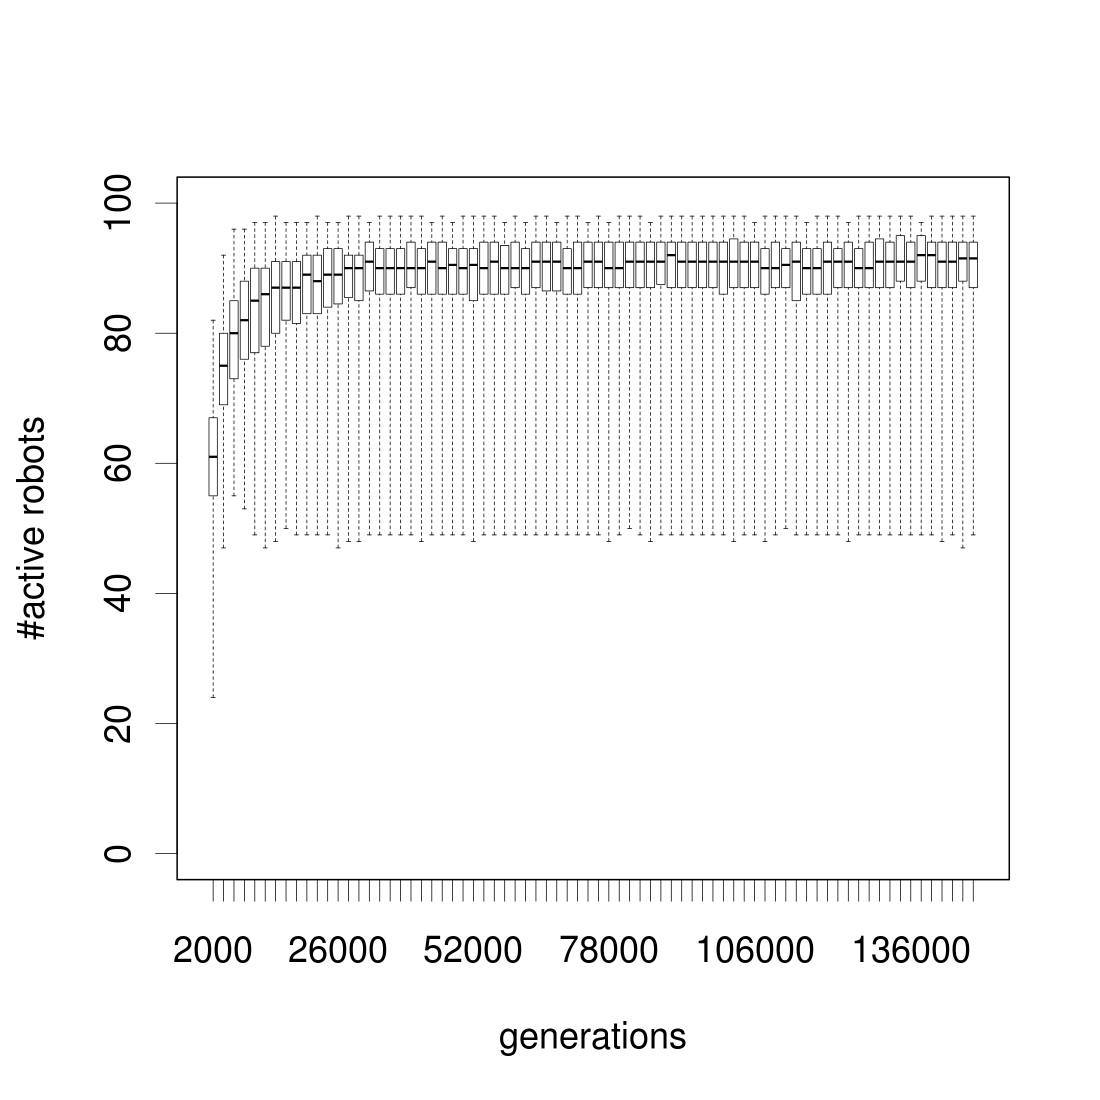
\includegraphics[width=\imgSize]{../images/5StaticEnv/alive_staticEnv1}& 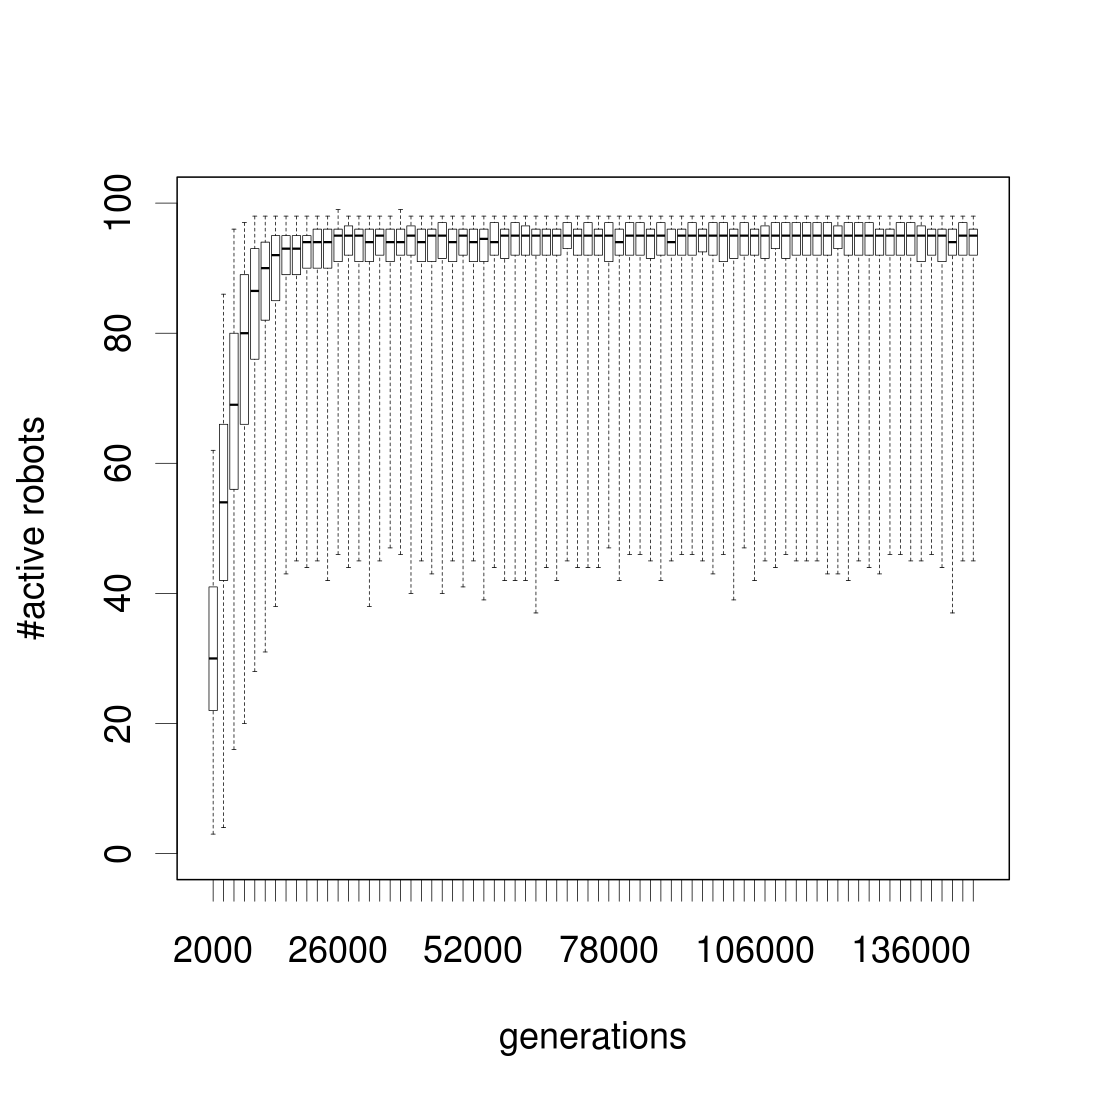
\includegraphics[width=\imgSize]{../images/5StaticEnv/alive_staticEnv2}\\ 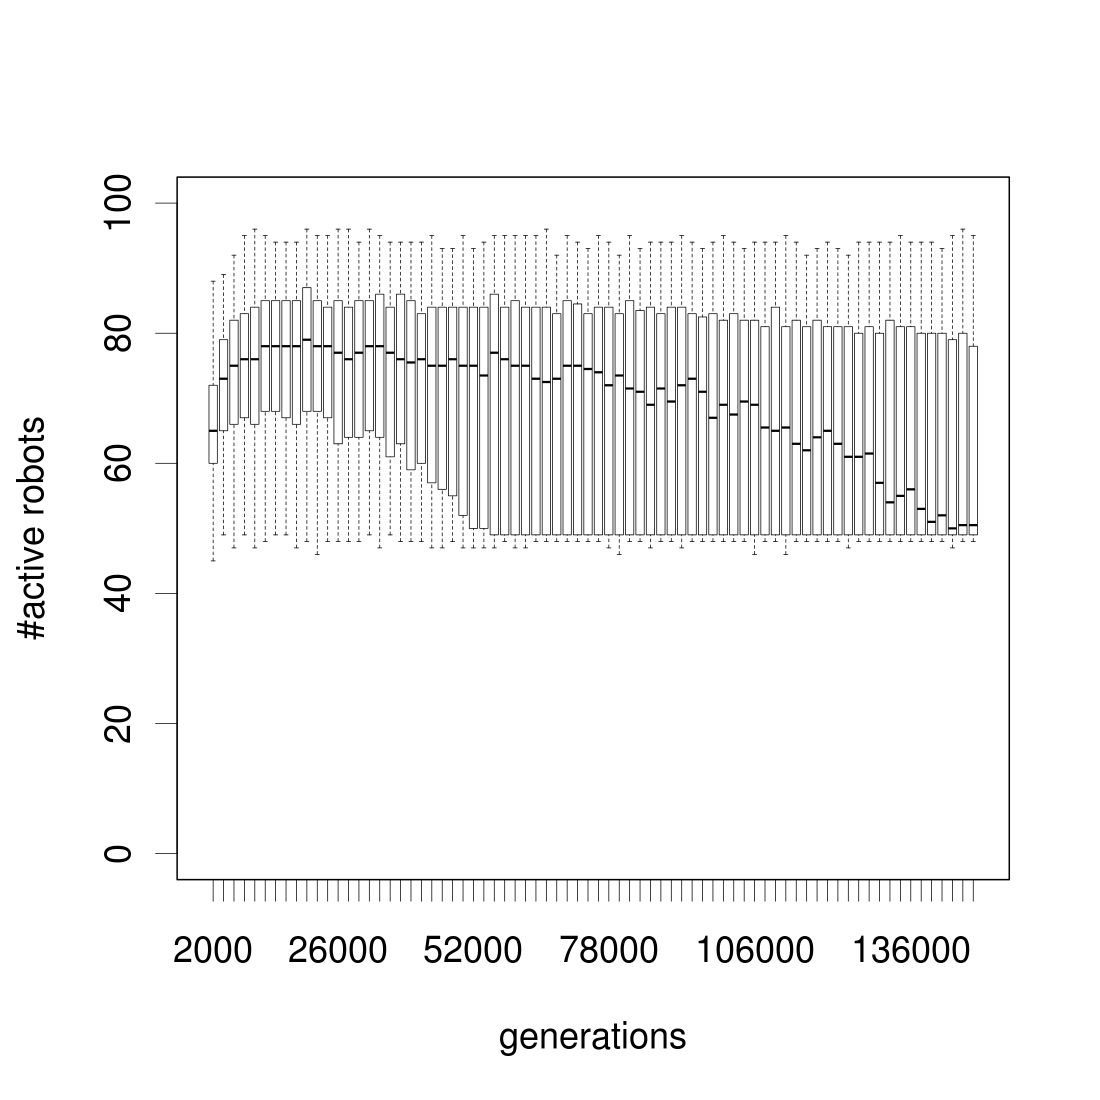
\includegraphics[width=\imgSize]{../images/5StaticEnv/alive_staticEnv0}& 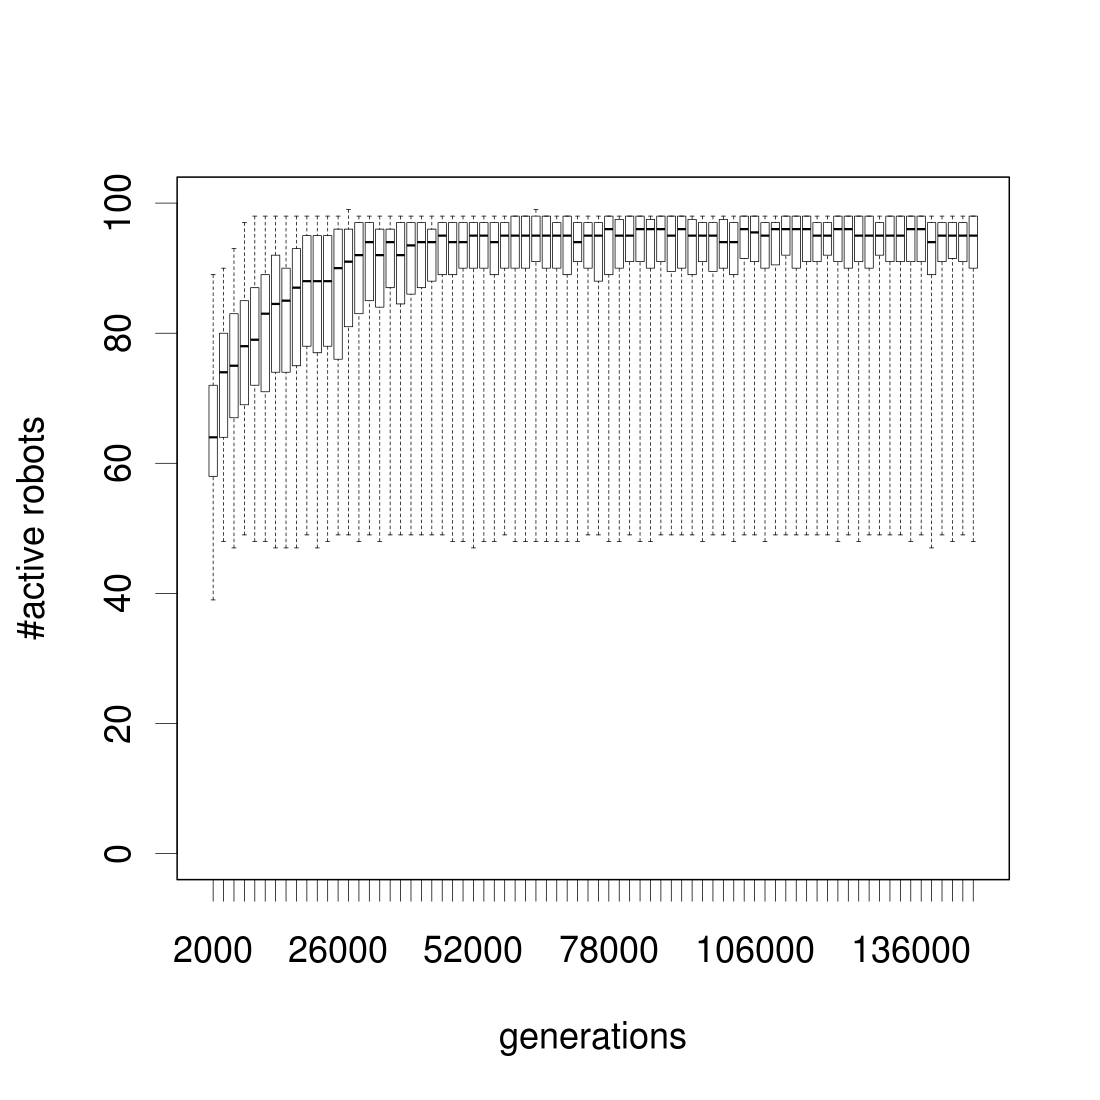
\includegraphics[width=\imgSize]{../images/5StaticEnv/alive_staticEnv3}& 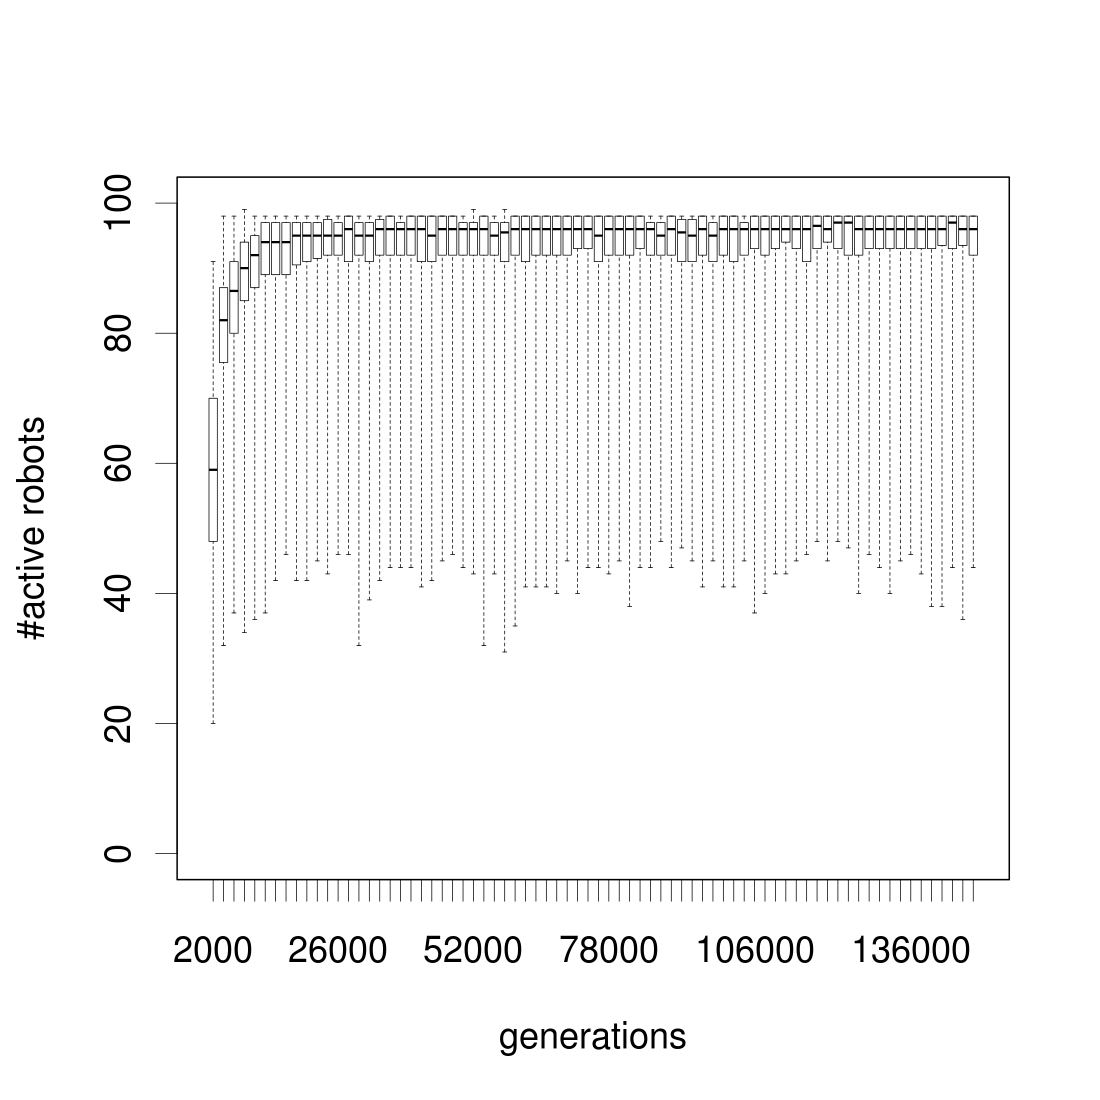
\includegraphics[width=\imgSize]{../images/5StaticEnv/alive_staticEnv4}\\ ENV0&ENV3&ENV4 \newline \end{tabular} \end{table} % 	
% \e
nd{columns}

\end{frame}





\begin{frame}{ENV0}
	\begin{table}[H]
	\centering
		\begin{tabular}{cc}
		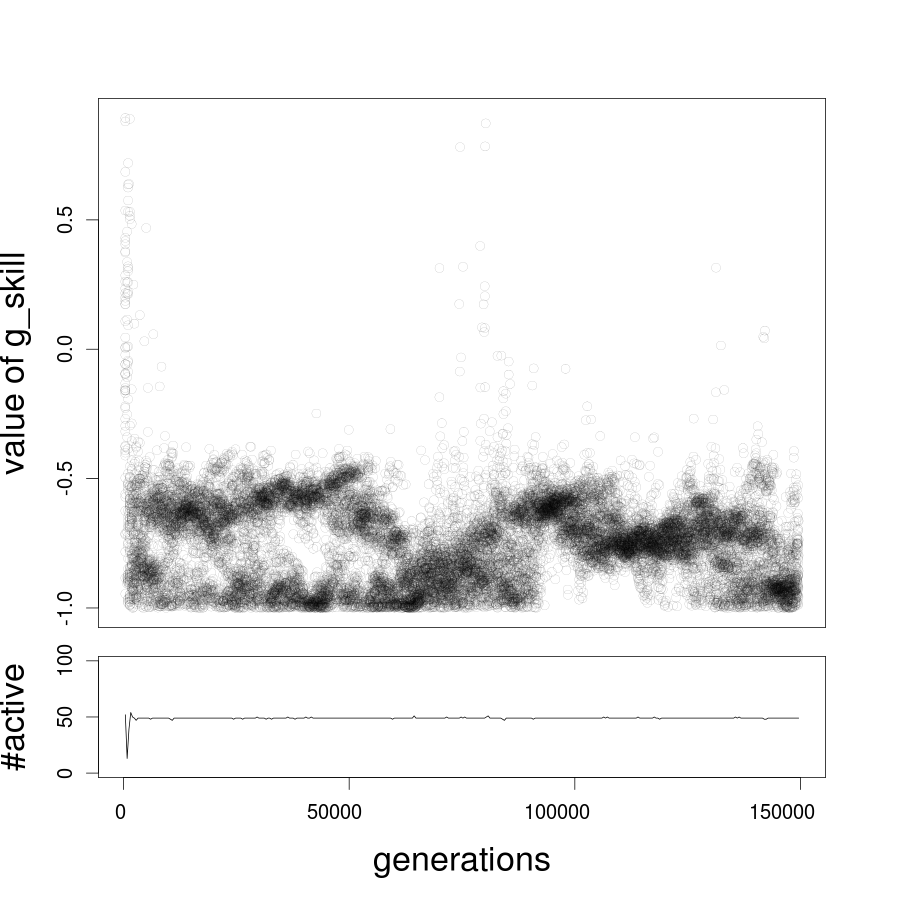
\includegraphics[width=\imgSize]{../images/5StaticEnv/Gplot62_staticEnv0}&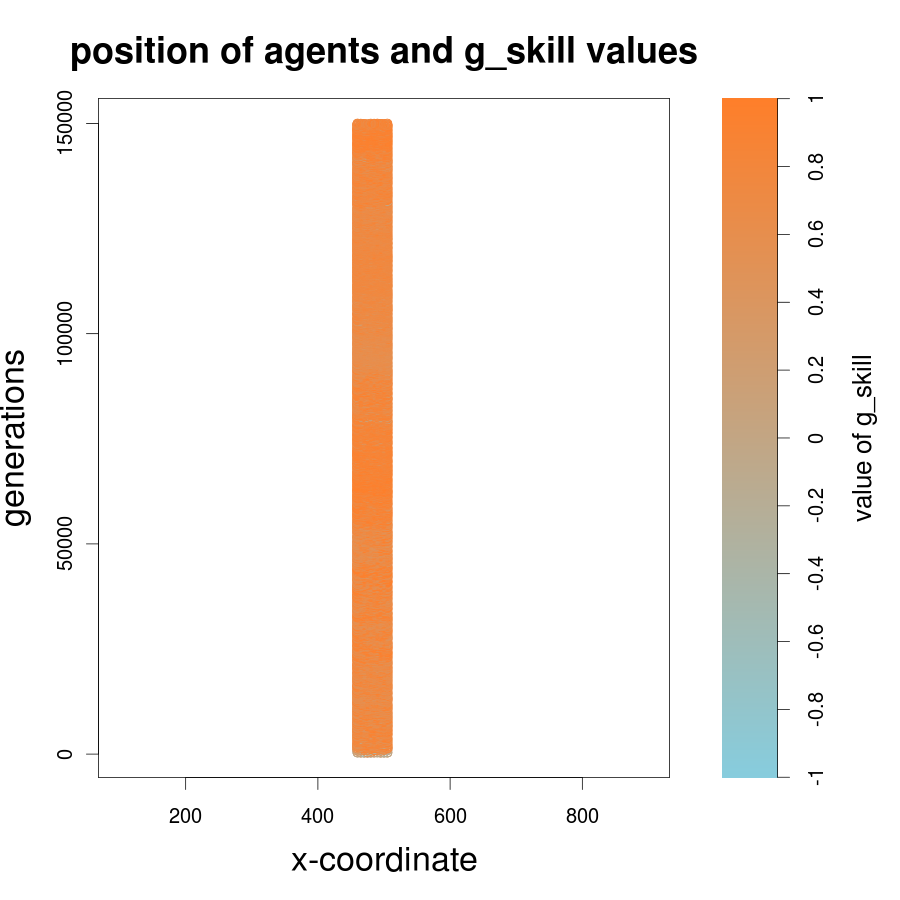
\includegraphics[width=\imgSize]{../images/5StaticEnv/Gplot62Static_staticEnv0}\\
		\newline
		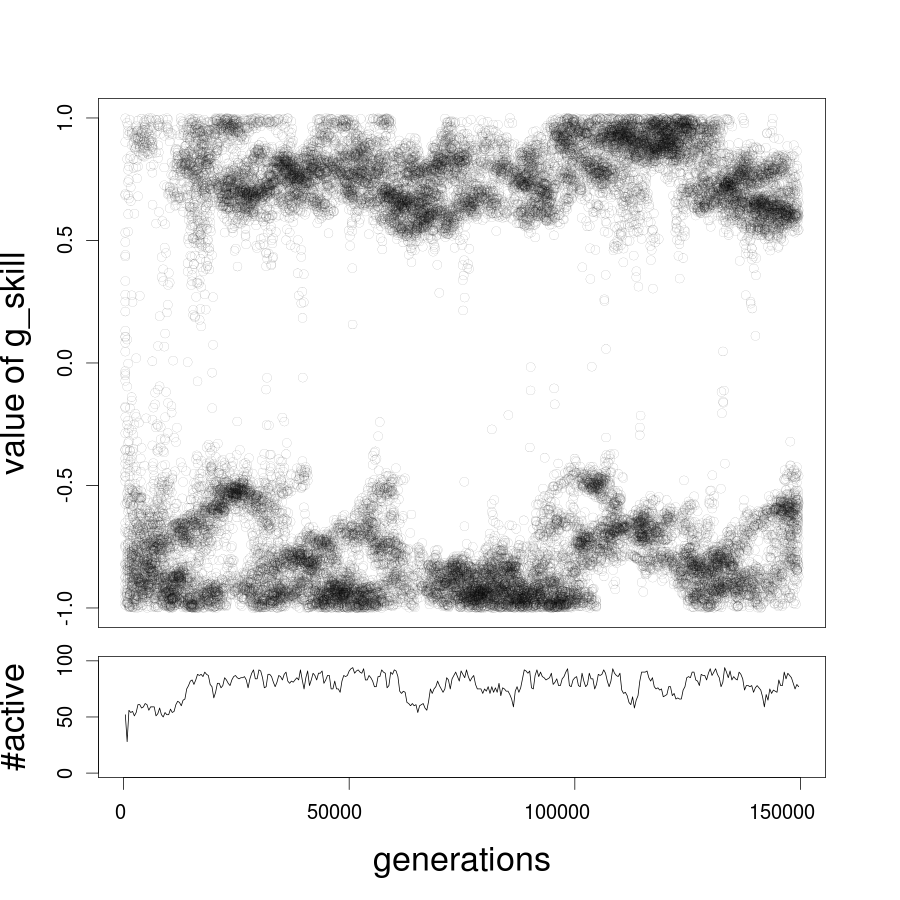
\includegraphics[width=\imgSize]{../images/5StaticEnv/Gplot58_staticEnv0}&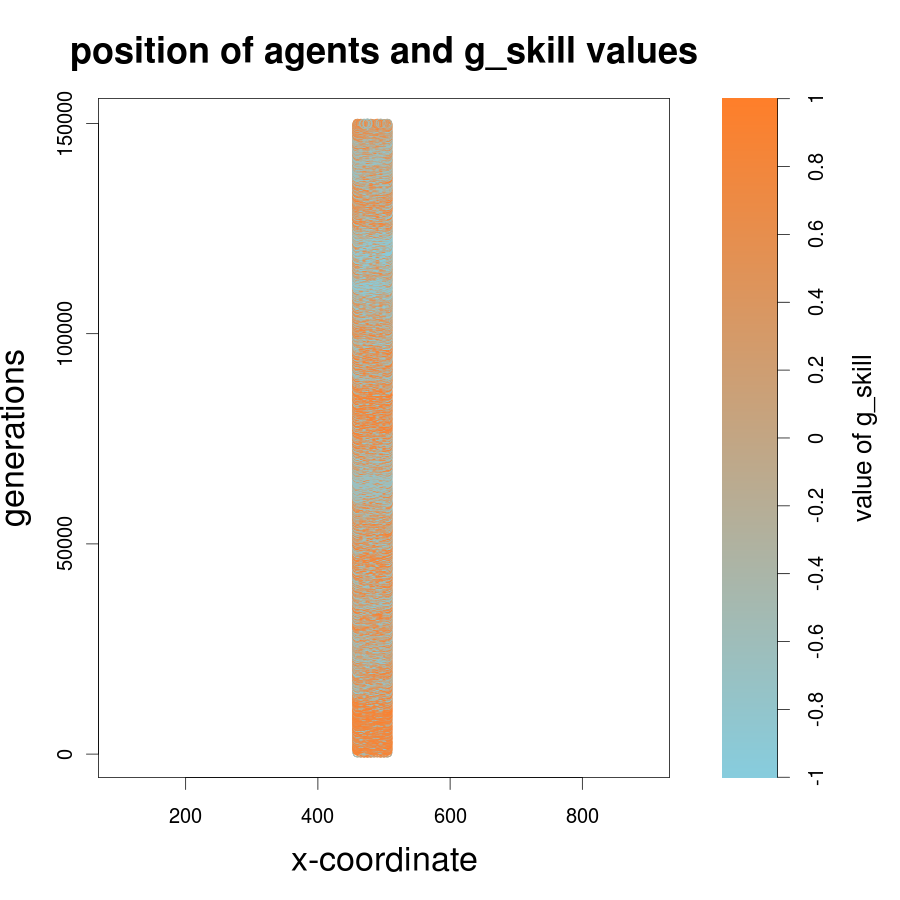
\includegraphics[width=\imgSize]{../images/5StaticEnv/Gplot58Static_staticEnv0}\\
		\end{tabular}
	\end{table}
\end{frame}
\begin{frame}{ENV1} \begin{table}[H] \centering \begin{tabular}{cc} 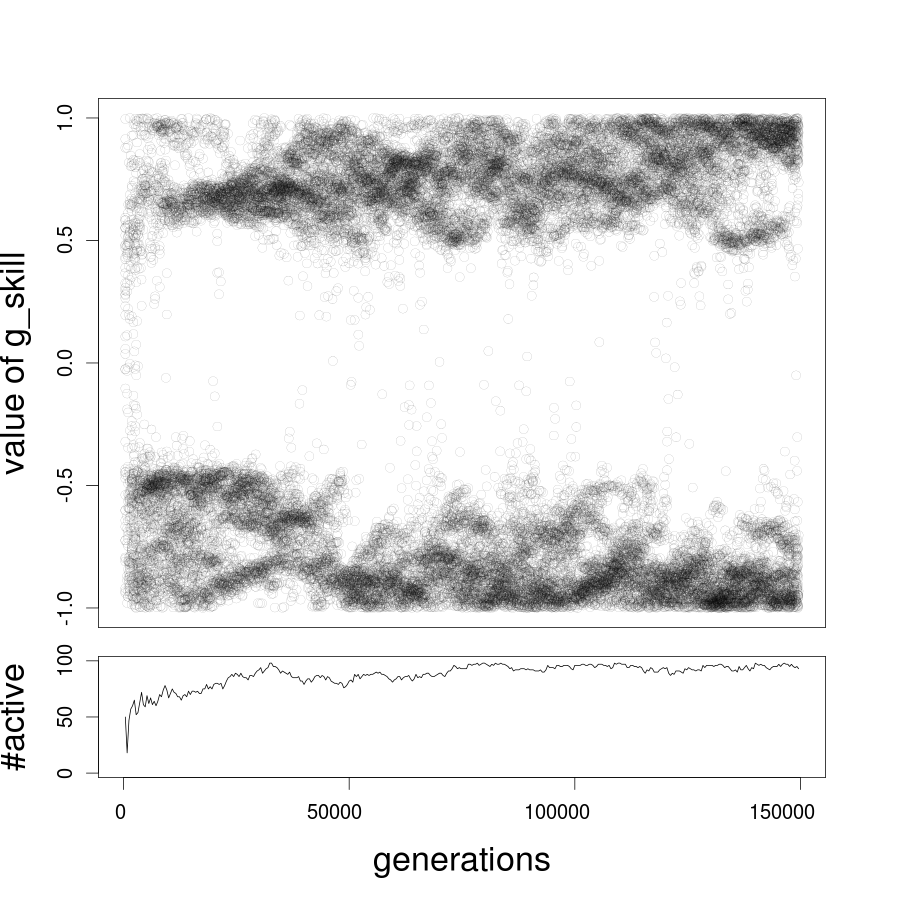
\includegraphics[width=\imgSize]{../images/5StaticEnv/Gplot47_staticEnv1}& 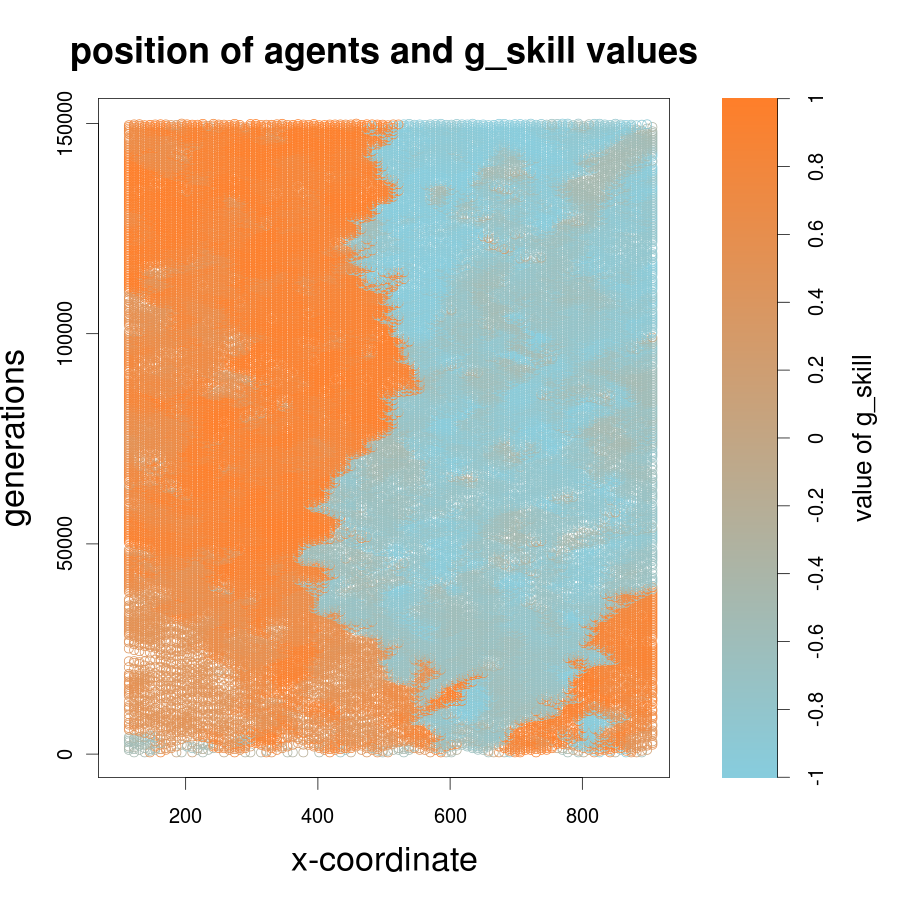
\includegraphics[width=\imgSize]{../images/5StaticEnv/Gplot47Static_staticEnv1}\\ \newline 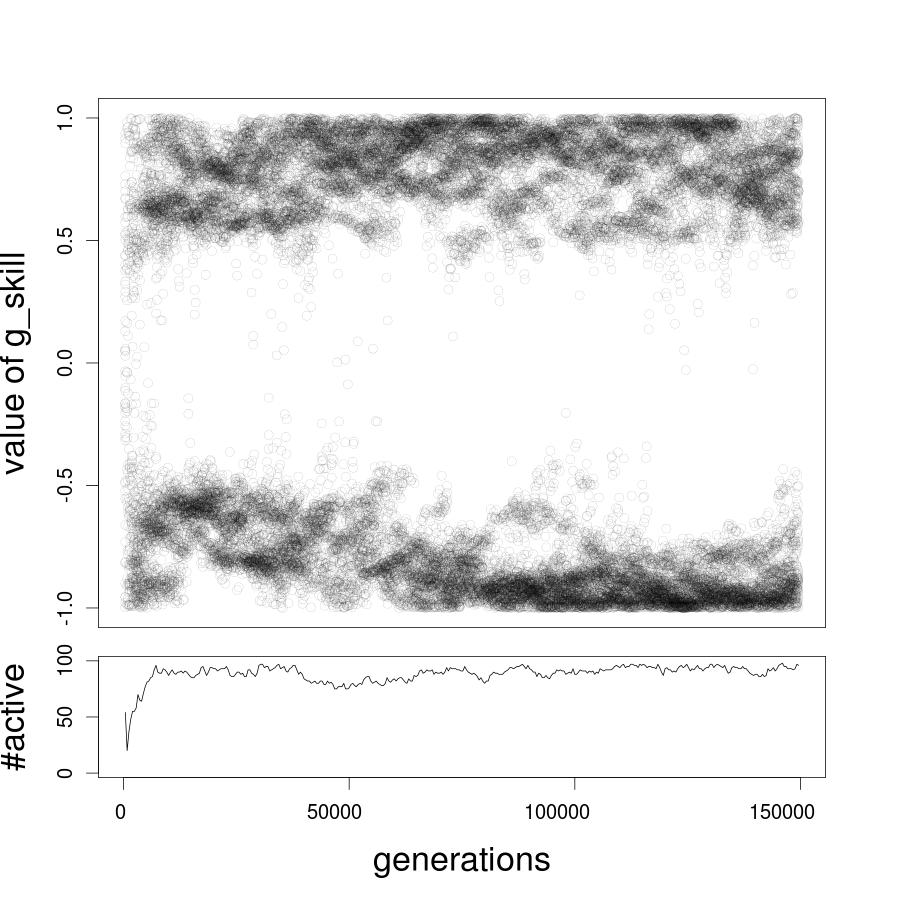
\includegraphics[width=\imgSize]{../images/5StaticEnv/Gplot29_staticEnv1}& 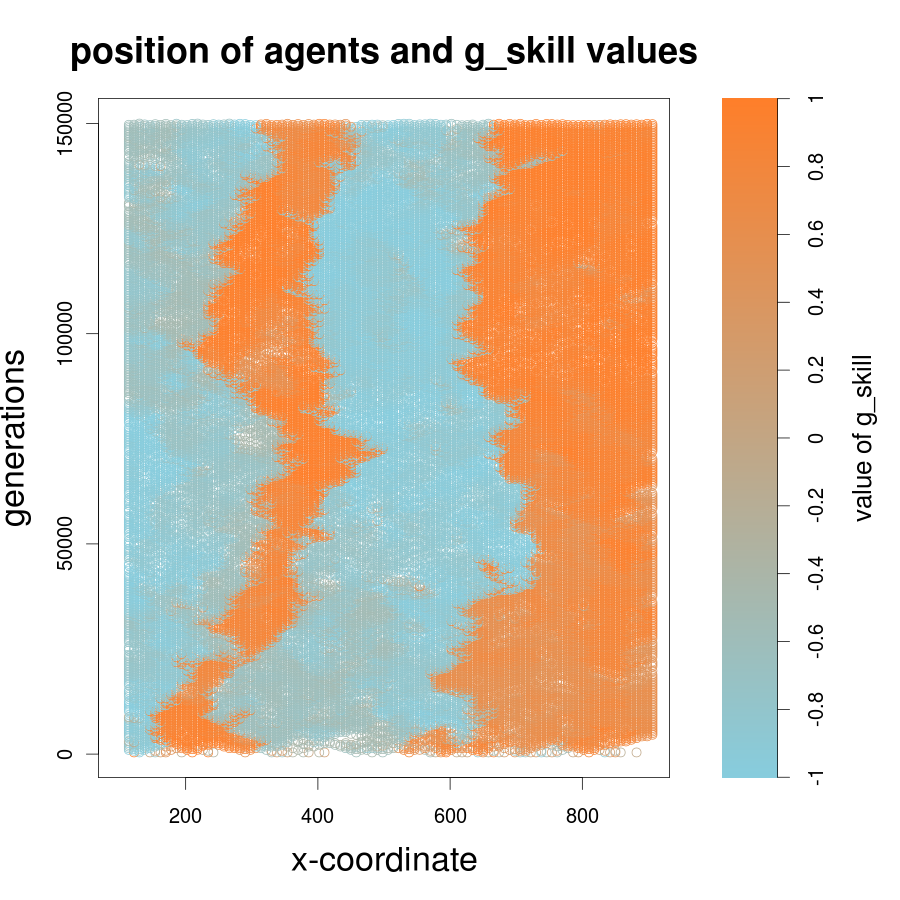
\includegraphics[width=\imgSize]{../images/5StaticEnv/Gplot29Static_staticEnv1}\\ \end{tabular} \end{table} \end{frame} \begin{frame}{ENV2} \begin{table}[H] \centering \begin{tabular}{cc} 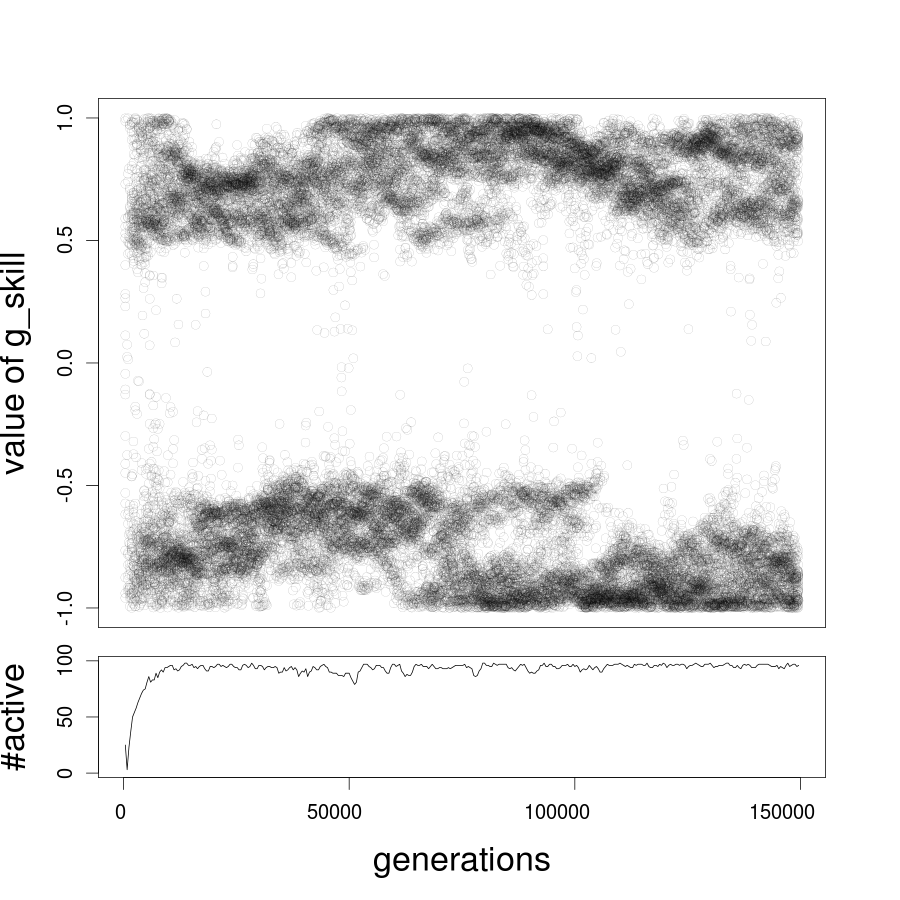
\includegraphics[width=\imgSize]{../images/5StaticEnv/Gplot22_staticEnv2}& 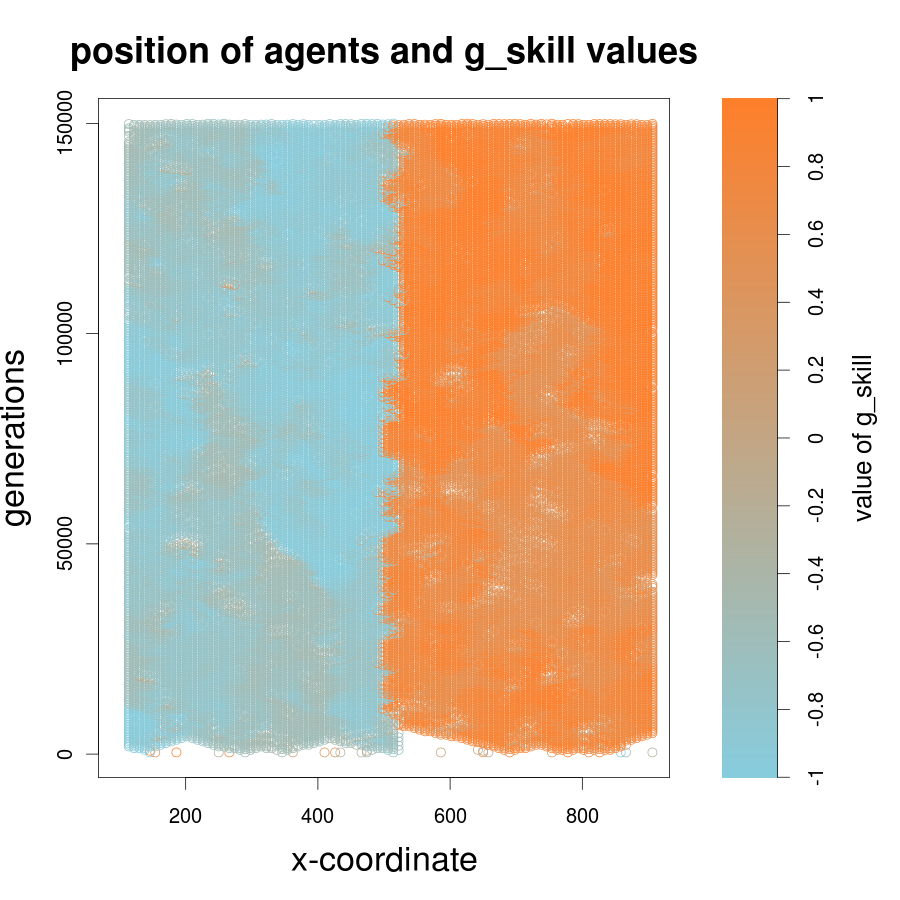
\includegraphics[width=\imgSize]{../images/5StaticEnv/Gplot22Static_staticEnv2}\\ 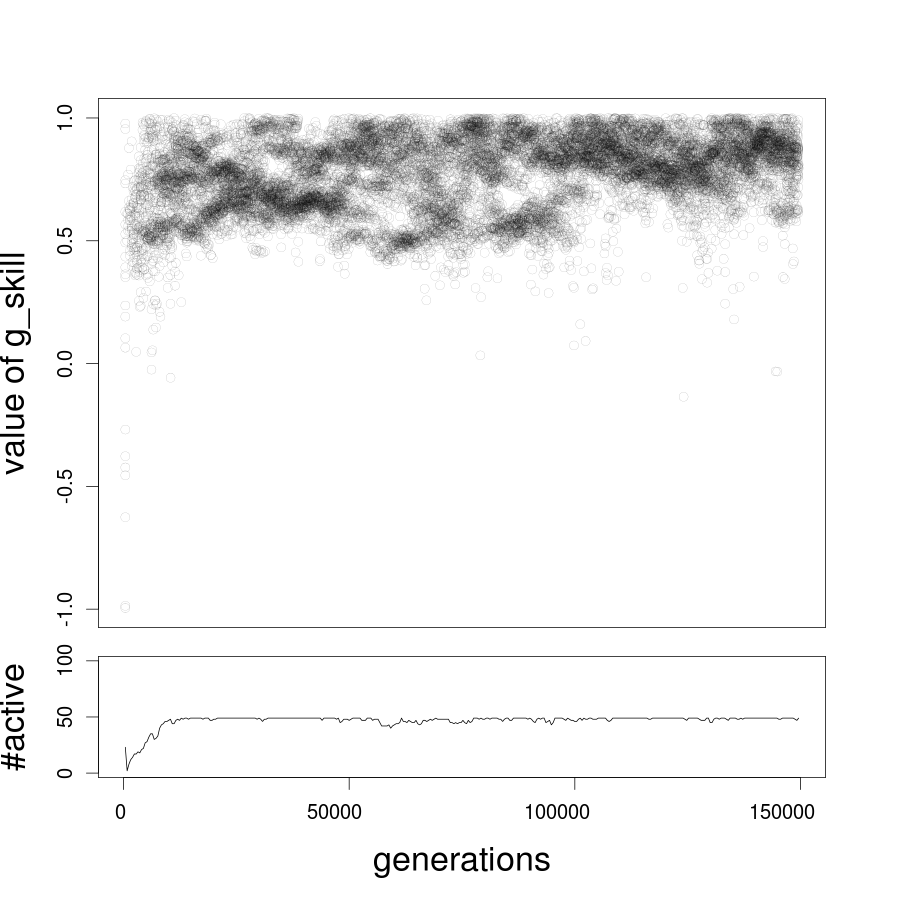
\includegraphics[width=\imgSize]{../images/5StaticEnv/Gplot92_staticEnv2}& 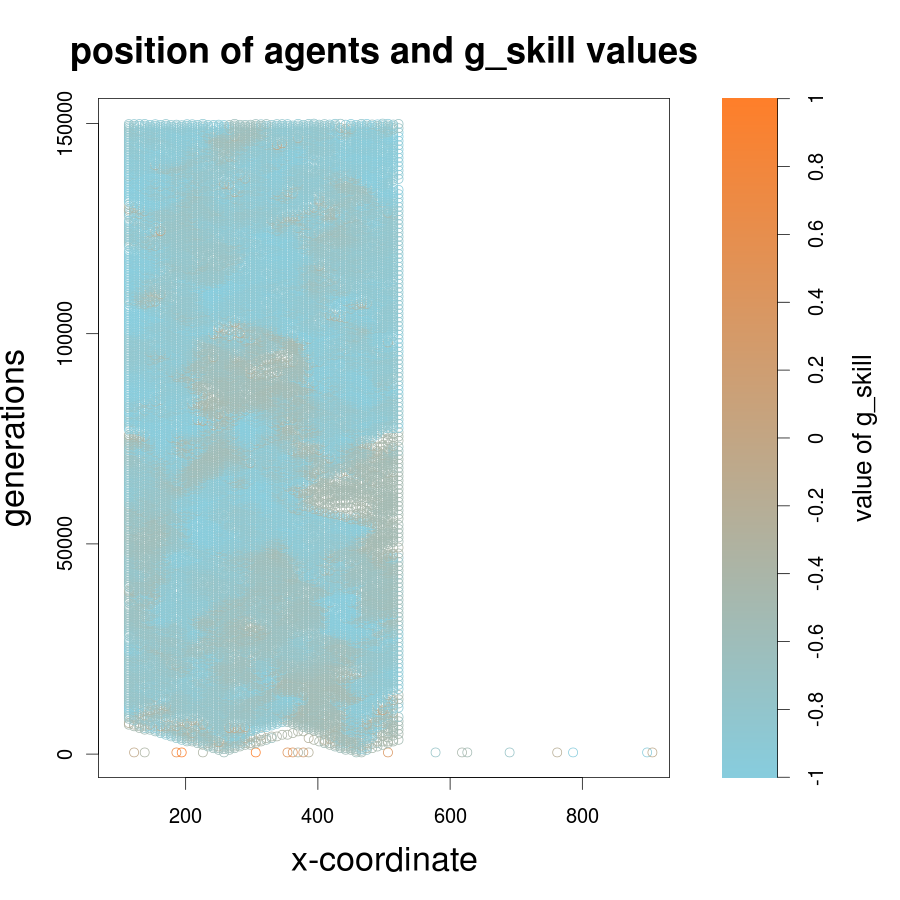
\includegraphics[width=\imgSize]{../images/5StaticEnv/Gplot92Static_staticEnv2}\\
		\end{tabular}
	\end{table}
\end{frame}



\begin{frame}{ENV3}
	\begin{table}[H]
		\centering
		\begin{tabular}{cc}
			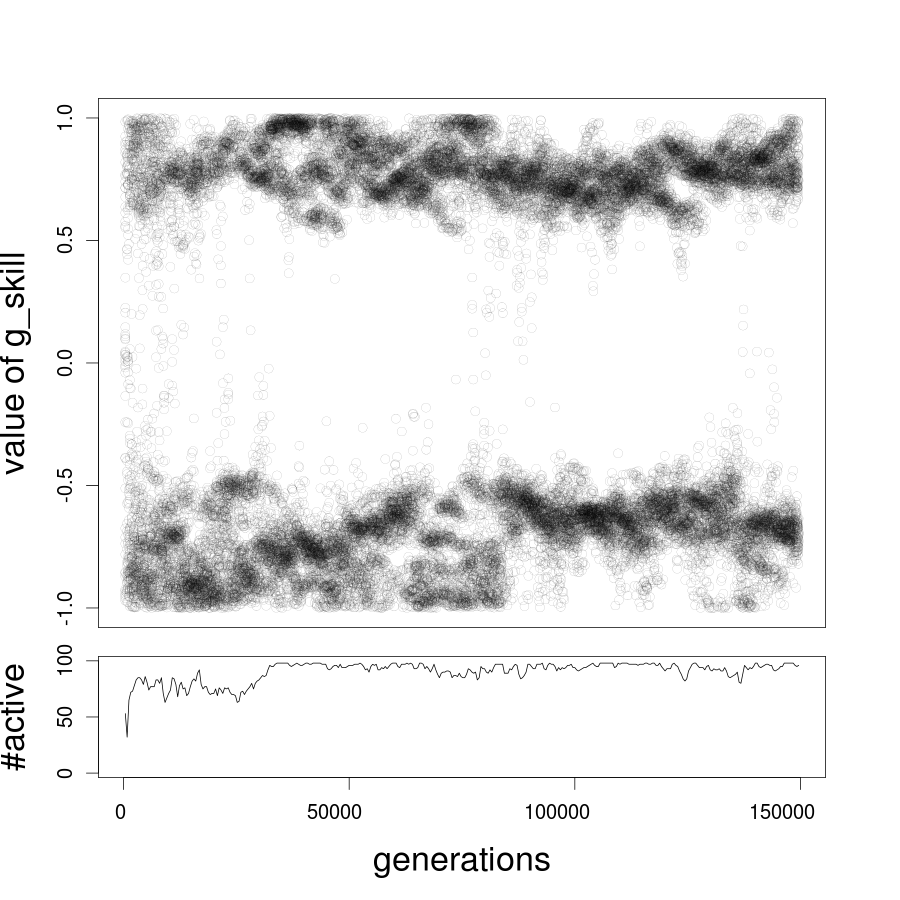
\includegraphics[width=\imgSize]{../images/5StaticEnv/Gplot5_staticEnv3}&
			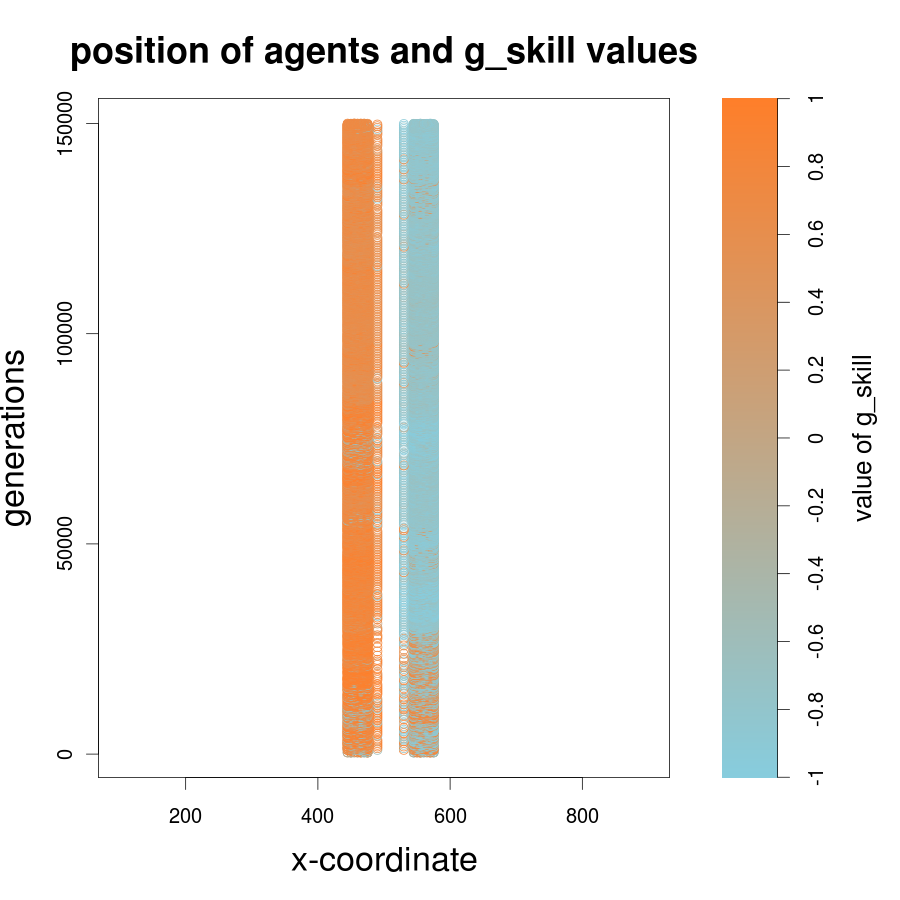
\includegraphics[width=\imgSize]{../images/5StaticEnv/Gplot5Static_staticEnv3}\\
			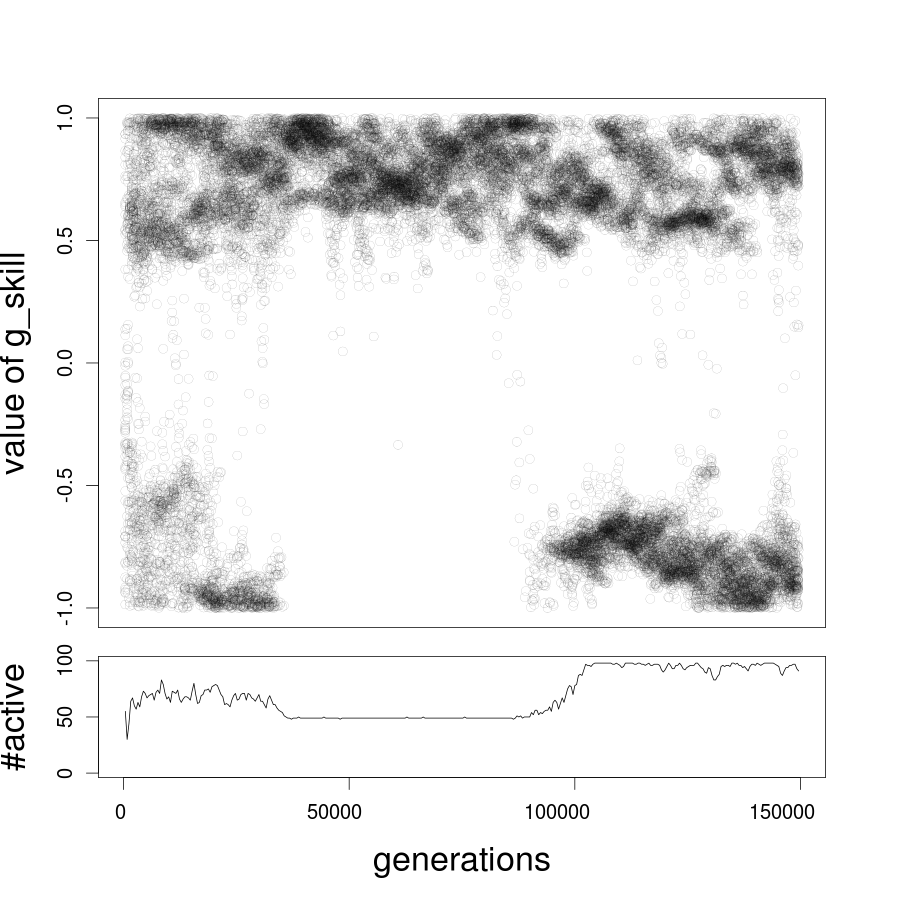
\includegraphics[width=\imgSize]{../images/5StaticEnv/Gplot99_staticEnv3}&
			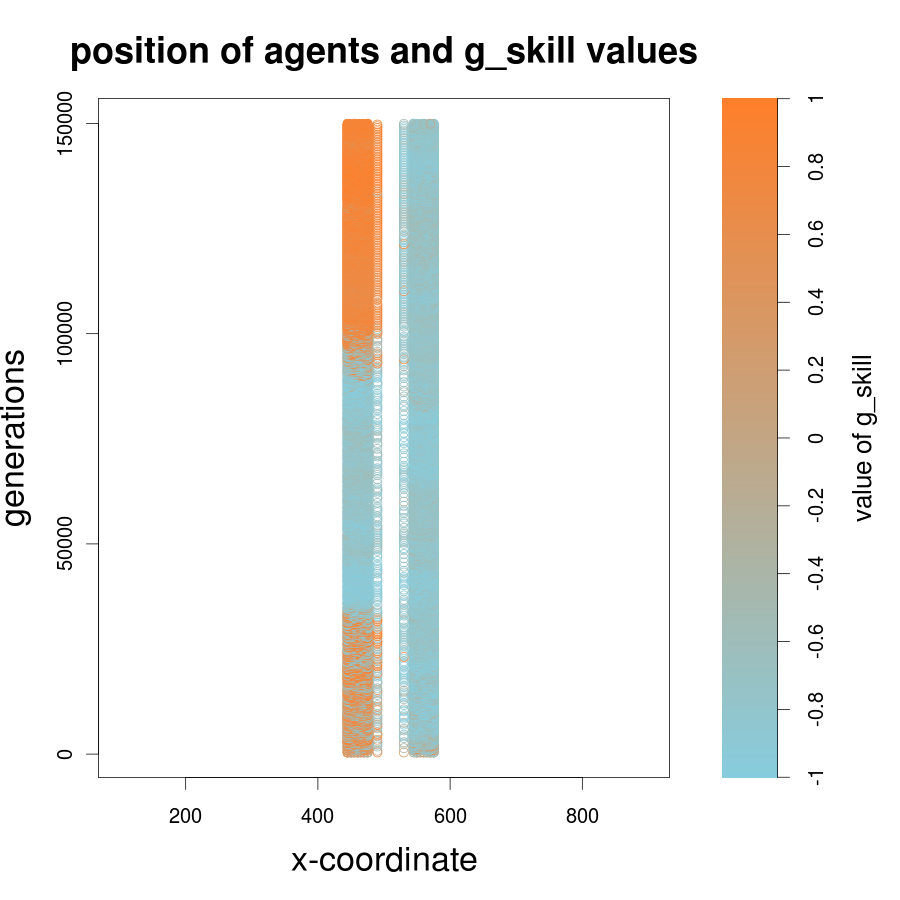
\includegraphics[width=\imgSize]{../images/5StaticEnv/Gplot99Static_staticEnv3}\\
		\end{tabular}
	\end{table}
\end{frame}




\begin{frame}{ENV4}
	\begin{table}[H]
		\centering
		\begin{tabular}{cc}
			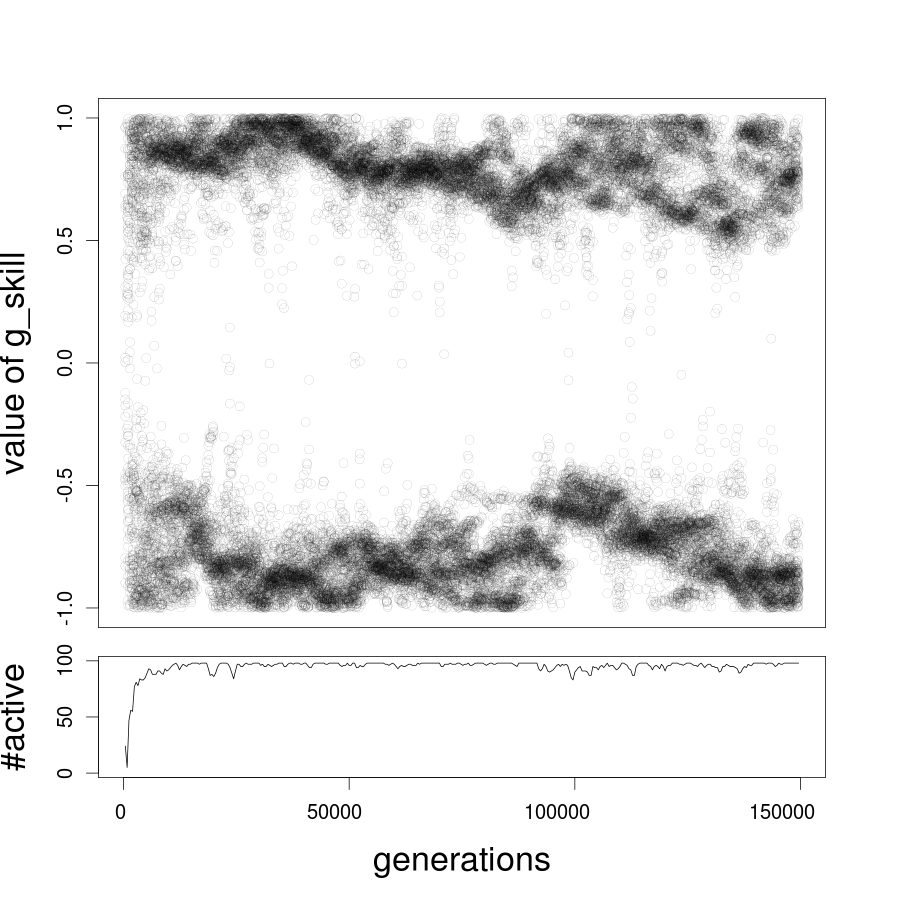
\includegraphics[width=\imgSize]{../images/5StaticEnv/Gplot62_staticEnv4}&
			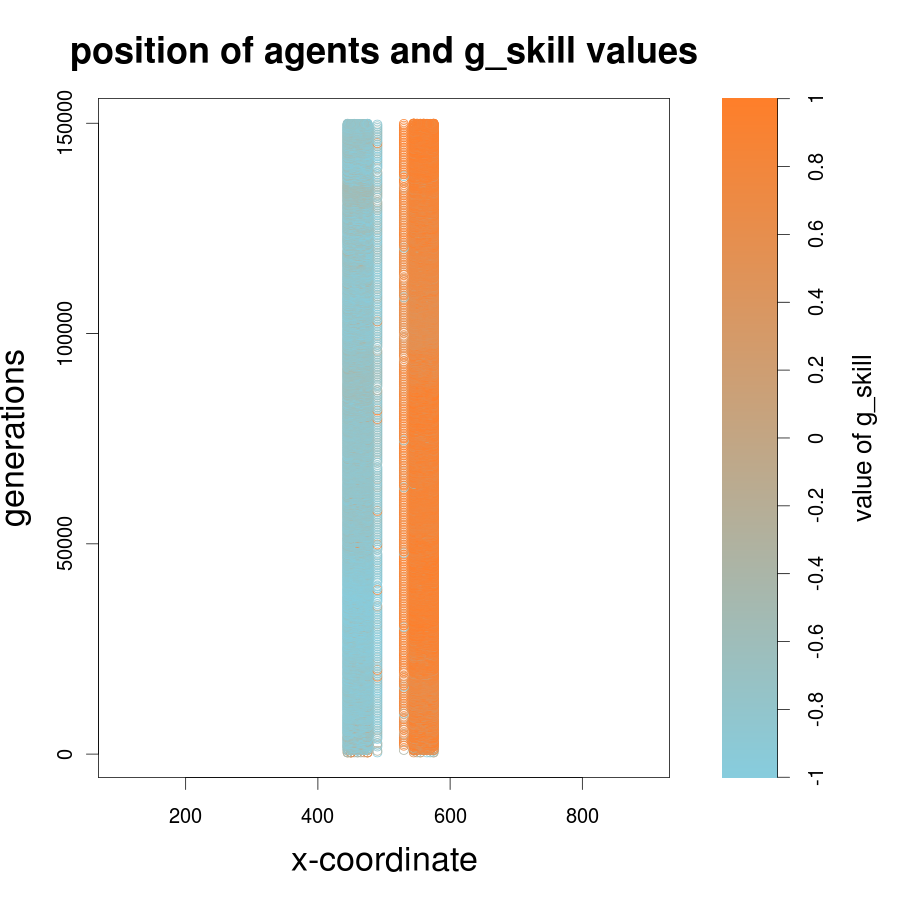
\includegraphics[width=\imgSize]{../images/5StaticEnv/Gplot62Static_staticEnv4}\\
			\newline
			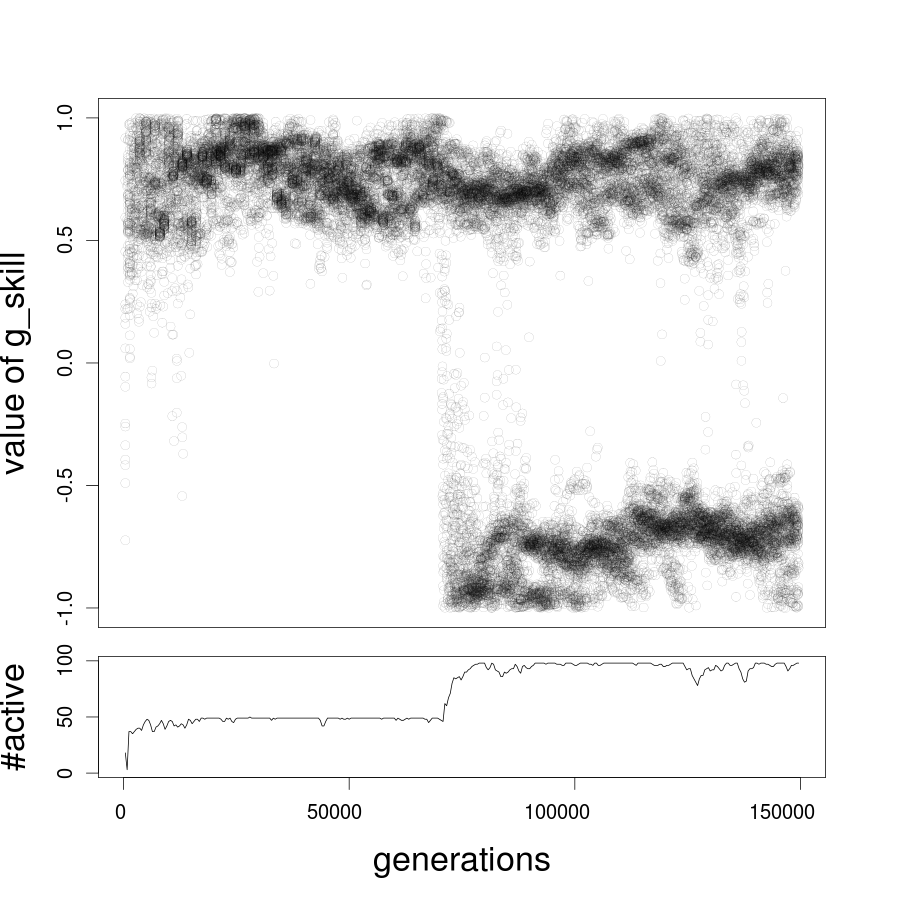
\includegraphics[width=\imgSize]{../images/5StaticEnv/Gplot40_staticEnv4}&
			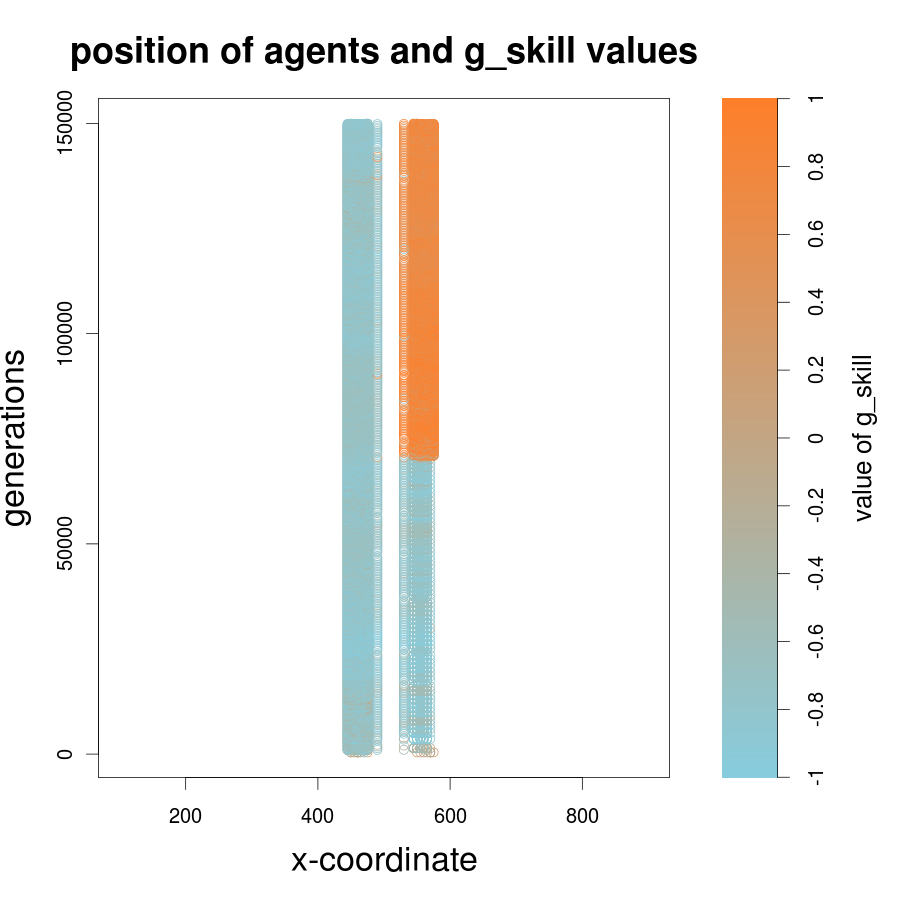
\includegraphics[width=\imgSize]{../images/5StaticEnv/Gplot40Static_staticEnv4}\\
		\end{tabular}
	\end{table}
\end{frame}

%%%----------------------------------------------------------------------
%%%----------------------------------------------------------------------
\subsubsection{Variable availablity}
\begin{frame}{}
	\begin{block}{Environmental variations}
		What if we change the ressources availabilities? 
		\begin{itemize}
		 \item Keep same robots dispositions and ressources access, 
		 \item But the amount of ressources available is not 50-50.
		\end{itemize}

	\end{block}
\end{frame}



\begin{frame}{ENV 1 \& ENV 2}
	\begin{table}[H]
	\centering
		\begin{tabular}{cc}
		ENV1&ENV2\\
		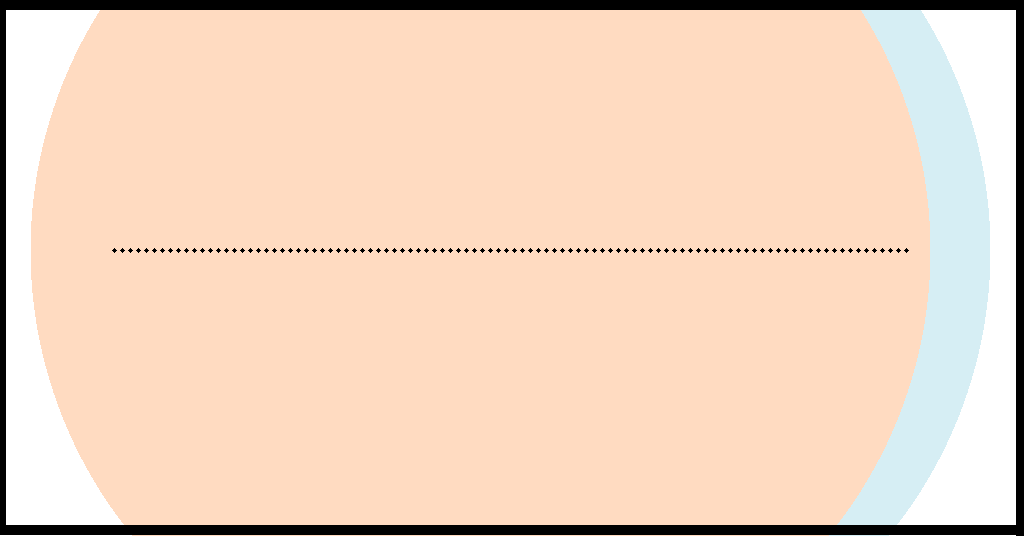
\includegraphics[width=2cm]{../images/5StaticEnv/environments/staticEnv1}&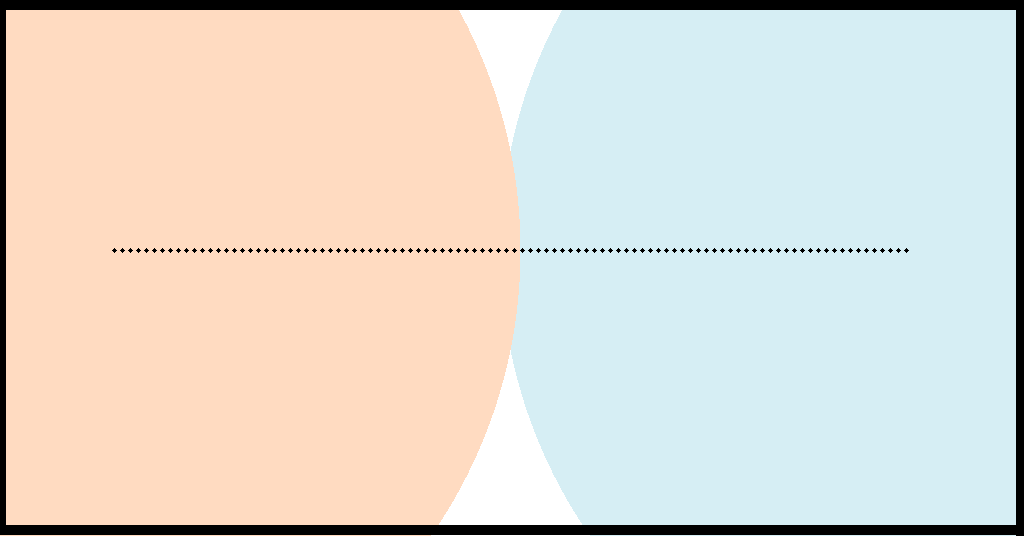
\includegraphics[width=2cm]{../images/5StaticEnv/environments/staticEnv2}\\
		\newline
		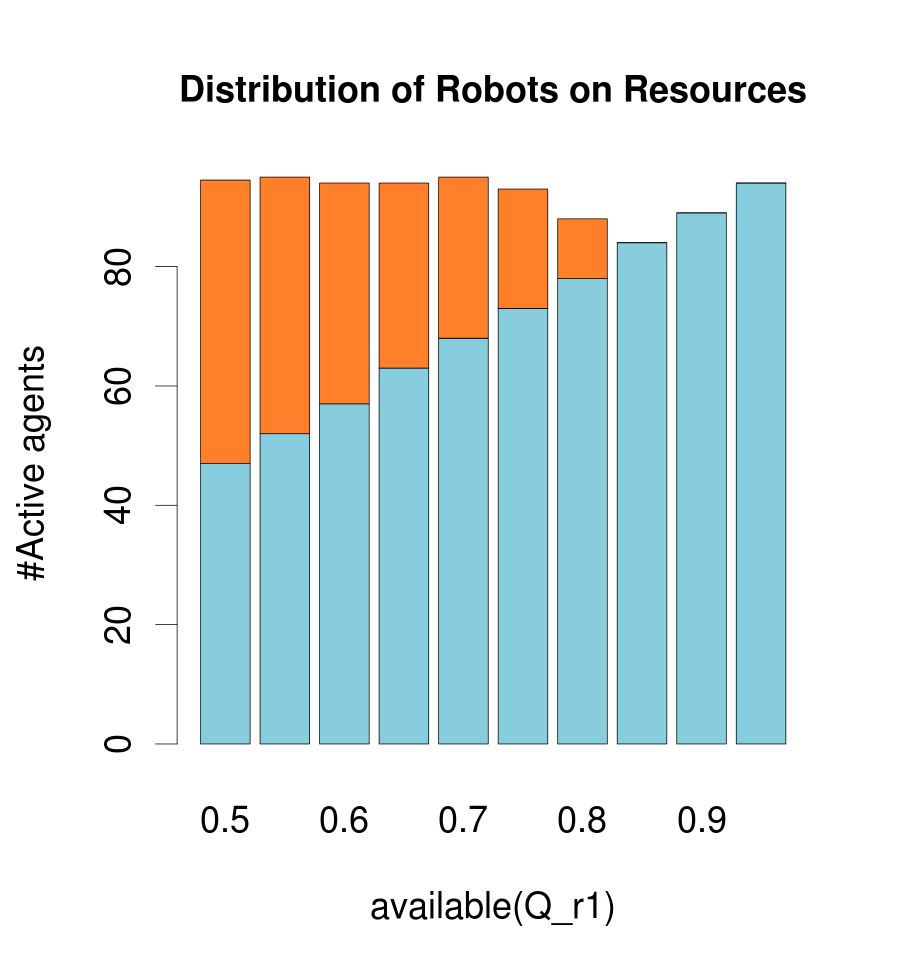
\includegraphics[width=\imgSize]{../images/5StaticEnv/barplotAliveR1AndR2_median_env1}&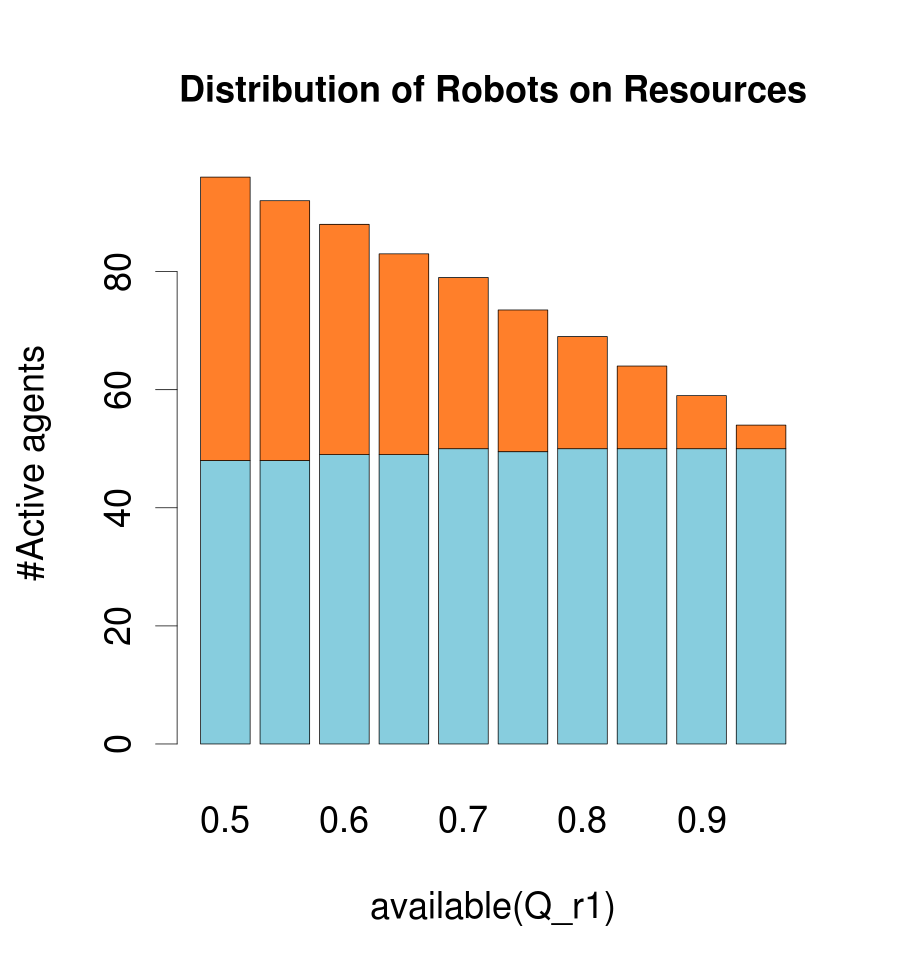
\includegraphics[width=\imgSize]{../images/5StaticEnv/barplotAliveR1AndR2_median_env2}\\
		\end{tabular}
	\end{table}
\end{frame}

\begin{frame}{ENV3 \& ENV4}
	\begin{table}[H]
		\centering
		\begin{tabular}{cc}
		ENV3 & ENV4\\
		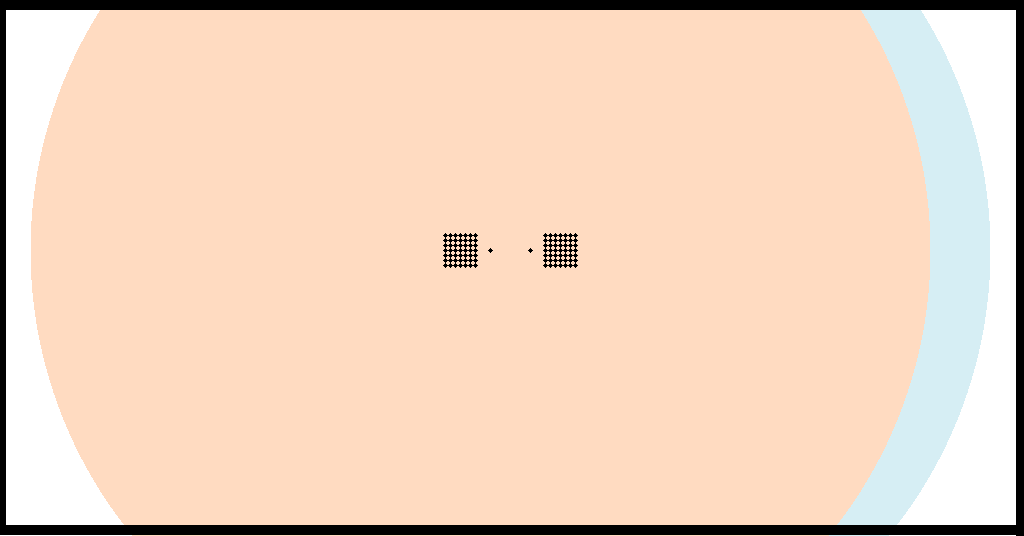
\includegraphics[width=3cm]{../images/5StaticEnv/environments/staticEnv3}&
		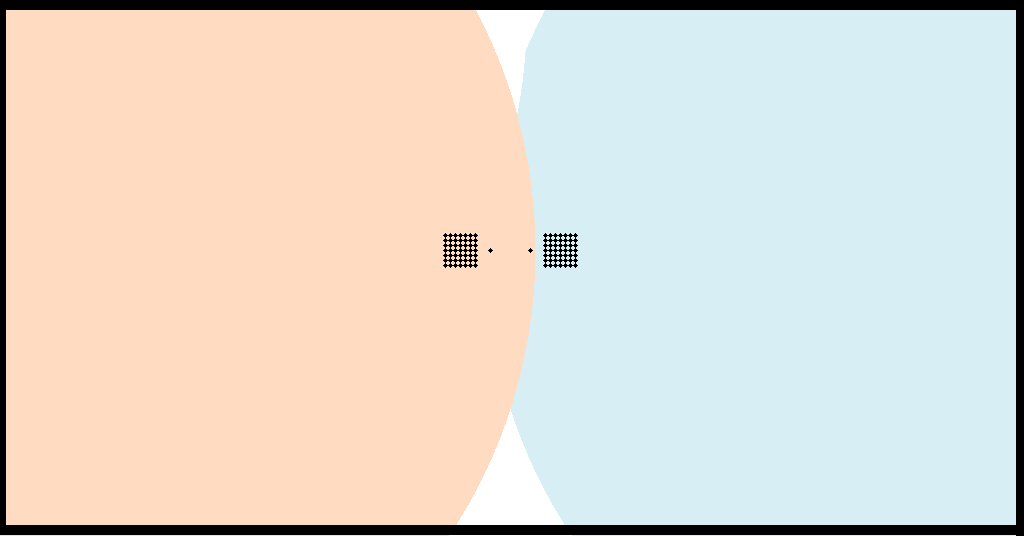
\includegraphics[width=3cm]{../images/5StaticEnv/environments/staticEnv4}\\
		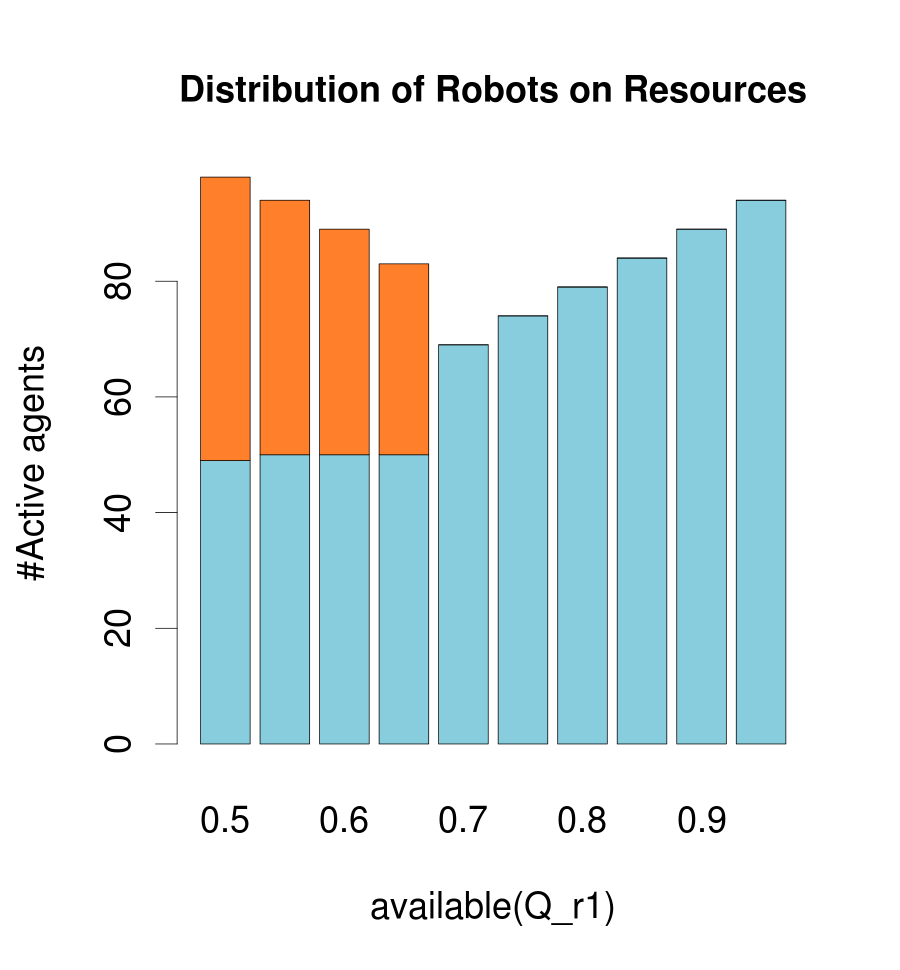
\includegraphics[width=\imgSize]{../images/5StaticEnv/barplotAliveR1AndR2_median_env3}&
		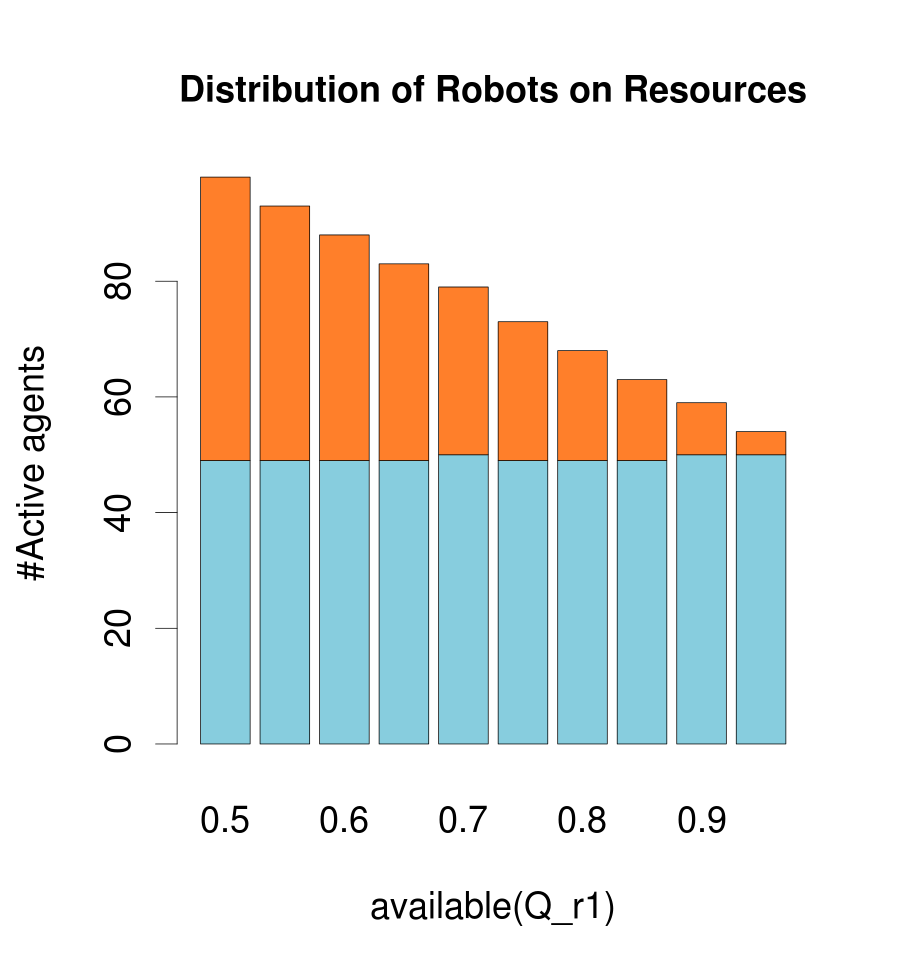
\includegraphics[width=\imgSize]{../images/5StaticEnv/barplotAliveR1AndR2_median_env4}
		\end{tabular}
	\end{table}
\end{frame}

\begin{frame}{ENV 0}

	\begin{table}[H]
		\begin{tabular}{cc}
			\includegraphics[width=\imgSize]{../images/5StaticEnv/environments/staticEnv0}&\\
			\includegraphics[width=\imgSize]{../images/5StaticEnv/barplotAliveR1AndR2_median_env0}\\
		\end{tabular}
	\end{table}
	% \vspace{-1cm}
\end{frame}
%%%----------------------------------------------------------------------
%%%----------------------------------------------------------------------



\section{Exhaustive analyse of the density's effect}
\subsection{Experimental design}

\begin{frame}{Density's effect}
	\renewcommand{\imgSize}{3cm}
	How the density of the communication's network affects speciation?

	\vfill
	\begin{columns}
		\column{0.3\textwidth}
			Density = $0.99$
		\column{0.3\textwidth}
			$0.50$
		\column{0.3\textwidth}
			$0.02$
	\end{columns}
	\vfill
	\begin{columns}
		\column{0.3\textwidth}
			\includegraphics[width=\imgSize]{images/networks/neato_Network_sparsity1}\\
		\column{0.3\textwidth}
			\includegraphics[width=\imgSize]{images/networks/neato_Network_sparsity50.png}\\
		\column{0.3\textwidth}
			\includegraphics[width=\imgSize]{images/networks/neato_Network_sparsity98.png}\\
	\end{columns}

\end{frame}



%%%----------------------------------------------------------------------
%%%----------------------------------------------------------------------
\subsection{Results}



\begin{frame}{Density's effect}
	\renewcommand{\imgSize}{3.8cm}

	\begin{table}[H]
		% \caption{pourcentage }
		\centering
		\begin{tabular}{cc}
			R1 & R0\\
			\includegraphics[width=\imgSize]{images/R1_median}&\includegraphics[width=\imgSize]{images/R0_median}\\
			\includegraphics[width=\imgSize]{images/active_median}\\
			Number of alive&\\
		\end{tabular}

	\end{table}

\end{frame}


\begin{frame}{ Slices through the density axis : }

	\renewcommand{\imgSize}{3.8cm}	
	\begin{table}[H]

		\centering
		\begin{tabular}{cc}
			density=.02&density=.08\\
			\includegraphics[width=\imgSize]{images/alive_r1_density-2.png}&
			\includegraphics[width=\imgSize]{images/alive_r1_density-8.png}\\
			\includegraphics[width=\imgSize]{images/alive_r1_density-60.png}&
			\includegraphics[width=\imgSize]{images/active_median}\\
			density=.6&\\
		\end{tabular}

	\end{table}

\end{frame}

\section{Conclusion}

\begin{frame}{Conclusion}
	\begin{block}{Using mEDEA}
		\begin{itemize}
			\item Speciation emerges in some particular environments.
			\item The range where speciation arise is small but large enough to allow us to put our system in it.
			\item Choose only some (first met) neighbours ? preference mating? 
		\end{itemize}
	\end{block}
\end{frame}

%%%----------------------------------------------------------------------
%%%----------------------------------------------------------------------
%%%----------------------------------------------------------------------
\begin{frame}%\addtocounter{framenumber}{-1}
\begin{center}
Merci pour votre attention.
\end{center}
\end{frame}

\begin{frame}{ slice through the density axis : }\addtocounter{framenumber}{-1}
\begin{figure}[H]
\includegraphics[width=\imgSize]{images/harvestr1_r1_density-2.png}
\includegraphics[width=\imgSize]{images/harvestr1_r1_density-8.png}\\
\includegraphics[width=\imgSize]{images/harvestr1_r1_density-60.png}
\includegraphics[width=\imgSize]{images/R1_median}

\end{figure}
\end{frame}

\renewcommand{\imgSize}{4cm}\addtocounter{framenumber}{-1}

\begin{frame}{slice through the $Q_{r1}$'s availablities axis : }
\begin{figure}[H]
\includegraphics[width=\imgSize]{images/alive_density_r1-50.png}
\includegraphics[width=\imgSize]{images/alive_density_r1-70.png}\\
\includegraphics[width=\imgSize]{images/alive_density_r1-90.png}
\includegraphics[width=\imgSize]{images/active_median}
\end{figure}

\end{frame}
\begin{frame}{slice through the $Q_{r1}$'s availablities axis : }\addtocounter{framenumber}{-1}

\begin{figure}[H]
\includegraphics[width=\imgSize]{images/harvestr1_density_r1-50.png}
\includegraphics[width=\imgSize]{images/harvestr1_density_r1-70.png}\\
\includegraphics[width=\imgSize]{images/harvestr1_density_r1-90.png}
\includegraphics[width=\imgSize]{images/R1_median}
\end{figure}
\end{frame}
\end{document}
		
